\documentclass[12pt]{article}

\usepackage[margin = 1in]{geometry}
\usepackage{graphicx}              
\usepackage{amsmath}               
\usepackage{amsfonts}              
\usepackage{amsthm}                
\usepackage{amssymb}
\usepackage{mathrsfs}
\usepackage{url}
\usepackage{subfig}
\usepackage{xfrac}
\usepackage[sectionbib]{chapterbib}
\usepackage{hyperref}
\usepackage{tikz}
\usetikzlibrary{positioning,calc,arrows}
\usepackage{algorithmic}
\usepackage{enumerate}

\hypersetup{
	unicode=true,
	colorlinks=true,
	citecolor=black,
	filecolor=black,
	linkcolor=black,
	urlcolor=black,
	pdfstartview={FitH},
}

% theorem environments
\theoremstyle{plain}
\newtheorem{theorem}{Theorem}
\newtheorem{lemma}[theorem]{Lemma}
\newtheorem{corollary}[theorem]{Corollary}
\newtheorem{proposition}[theorem]{Proposition}
\theoremstyle{definition}
\newtheorem{definition}[theorem]{Definition}
\newtheorem{conjecture}[theorem]{Conjecture}
\newtheorem{example}[theorem]{Example}
\newtheorem*{remark}{Remark}
\newtheorem{note}[theorem]{Note}


\renewcommand{\algorithmicrequire}{\textbf{Input:}}
\renewcommand{\algorithmicensure}{\textbf{Output:}}
\algsetup{linenodelimiter=.}

\newcommand{\wrt}{\vdash} 
\newcommand{\ang}[1]{\langle#1\rangle}
\newcommand{\abs}[1]{\left\vert#1\right\vert}
\newcommand{\dual}[1]{\overline{#1}}
\newcommand{\mapsfrom}{\ensuremath{\reflectbox{$\mapsto$}}}
\newcommand{\tildO}{\tilde{O}}
% roman numerals
\newcommand{\romnum}[1]{\romannumeral #1}
\newcommand{\Romnum}[1]{\uppercase\expandafter{\romannumeral #1}}

\newcommand{\todo}[1]{\textcolor{red}{TODO: #1}}
\newcommand{\comment}[2][Note]{\textcolor{green}{(#1): #2}}

\DeclareMathOperator{\fieldchar}{char} % characteristic of a field
\DeclareMathOperator{\ringofend}{End} % endomorphism ring
\DeclareMathOperator{\trace}{Tr} % finite field trace
\DeclareMathOperator{\gal}{Gal} % Galois group
\DeclareMathOperator{\order}{ord} % order of an element
\DeclareMathOperator{\lcm}{lcm} % least common multiple
\DeclareMathOperator{\divisor}{div} % divisor on a curve
\DeclareMathOperator{\supp}{supp} % support of a divisor
\DeclareMathOperator{\norm}{N} % norm
\DeclareMathOperator{\Res}{Res}
\DeclareMathOperator{\Aut}{Aut}
\DeclareMathOperator{\minpoly}{minpoly}

\def\Q{\ensuremath{\mathbb{Q}}}
\def\N{\ensuremath{\mathbb{N}}}
\def\R{\ensuremath{\mathbb{R}}}
\def\Z{\ensuremath{\mathbb{Z}}}
\def\F{\ensuremath{\mathbb{F}}}
\def\H{\ensuremath{\mathbb{H}}}
\def\K{\ensuremath{\mathbb{K}}}
\def\L{\ensuremath{\mathbb{L}}}
\def\A{\ensuremath{\mathbb{A}}}
\def\B{\ensuremath{\mathbb{B}}}
\def\MM{\ensuremath{\mathsf{M}}}
\def\MMM{\ensuremath{\mathsf{MM}}}
\def\MC{\ensuremath{\mathsf{C}}}
\def\PC{\ensuremath{\mathsf{PC}}}
\def\II{\ensuremath{\mathsf{I}}}
\def\QQ{\ensuremath{\mathsf{Q}}}
\def\CC{\ensuremath{\mathsf{C}}}
\def\RR{\ensuremath{\mathsf{R}}}
\def\AA{\ensuremath{\mathsf{A}}}
\def\va{\ensuremath{\mathsf{a}}}
\def\vy{\ensuremath{\mathsf{y}}}
\def\vu{\ensuremath{\mathsf{u}}}
\def\vb{\ensuremath{\mathsf{b}}}
\def\vc{\ensuremath{\mathsf{c}}}
\def\mul{\ensuremath{\mathsf{mul}}}
\def\rem{\ensuremath{\mathsf{rem}}}
\def\cat{\ensuremath{\mathsf{cat}}}
\def\coeff{\ensuremath{\mathsf{coefficient}}}
\def\mulmod{\ensuremath{\mathsf{mulmod}}}
\def\rev{\ensuremath{\mathsf{rev}}}
\def\x{\ensuremath{\mathbf{x}}}
\def\uu{\ensuremath{\mathbf{U}}}
\def\bb{\ensuremath{\mathbf{B}}}
\def\bxi{\boldsymbol{\xi}}
\def\bupsilon{\boldsymbol{\upsilon}}
\def\bzeta{\boldsymbol{\zeta}}
\def\blambda{\boldsymbol{\lambda}}
\def\euler{\ensuremath{\varphi}}

% allow algorithms to split over multiple pages
\makeatletter
\newcounter{algorithm}
\setcounter{algorithm}{0}
\renewcommand{\thealgorithm}{\arabic{algorithm}}
\def\algorithm{\@ifnextchar[{\@algorithma}{\@algorithmb}}
\def\@algorithma[#1]{%
	\refstepcounter{algorithm}
	\trivlist
	\leftmargin\z@
	\itemindent\z@
	\labelsep\z@
	\item[\parbox{\columnwidth}{%
		\hrule
		\hrule
		\noindent\strut\textbf{Algorithm \thealgorithm} #1
		\hrule
	}]\hfil\vskip0em%
}
\def\@algorithmb{\@algorithma[]}
\def\endalgorithm{\hfil\vskip-1em\hrule\endtrivlist}
\makeatother


\title{Computing isomorphisms and embeddings of finite fields}
\author{Ludovic Brieulle, Luca De Feo, Javad Doliskani,\\ Jean-Pierre
  Flori and \'Eric Schost}


\begin{document}

\maketitle
\begin{abstract}
  Let $\F_q$ be a finite field.  The finite field embedding problem
  asks, given two irreducible polynomials $f,g$ over $\F_q$ with $\deg
  f$ dividing $\deg g$, to compute an explicit description of a field
  embedding of $\F_q[X]/f(X)$ into $\F_q[Y]/g(Y)$. When $\deg f = \deg
  g$, this is also known as the isomorphism problem.
  
  We review classical algorithms for the two problems, and compare
  their asymptotic complexities. We also propose new improvements and
  generalizations to the algorithms, implement them, and compare them
  with the state of the art.
\end{abstract}

\setcounter{tocdepth}{2}
\tableofcontents

%%%%%%%%%%%%%%%%%%%%%%%%%%%%%%%%%%
%%%%%%%%%%%%%%%%%%%%%%%%%%%%%%%%%%

\section*{Proposed notation}

This section is for internal reference only: erase after the paper has
stabilized.

\begin{itemize}
\item Base field: $\F_q$. Characteristic: $p$ (use it as little as
  possible). When algorithms only apply if $p=q$, state explicitly
  (verbally) that $q$ is prime.
\item Quotient notation: $\F_q[X]/f(X)$ or $\F_q[X]/(X^a-b)$, or
  $\F_q[X,Y]/(X^3,Y^6)$.
\item Other fields: $k = \F_q[X]/f(X)$, $K = \F_q[Y]/g(Y)$.
\item $m = \deg f, n=\deg g$, $m|n$.
\item $r$ a prime power dividing $m$.
\item $\phi,\psi$ embeddings.
\item Field trace $\trace$.
\item $\euler$: Euler function.
\item $\Phi_r$ cyclotomic polynomial, also modular polynomial.
\item $h$: factor of the cyclotomic polynomial.
\item Elliptic curves: $E:y^2=x^3+ax+b$ or $E:y^2+a_1xy+a_3y=x^3+\cdots$.
\item $\psi_m$ division polynomial, $\omega$ invariant differential.
\item $\pi$ frobenius endomorphism (elliptic curves), $t$ its trace,
  $\lambda,\mu$ its eigenvalues.
\item $s$ order of $q$ mod $r$ (Kummer), degree of auxiliary extension (Rains).
\item $\ell$ prime (power) such that $r|\order_\ell q$ (Rains).
\item modular integers: $\Z/m\Z$,
\item multiplicative groups: $\F_q^\ast$ and $(\Z/m\Z)^\ast$.
\item $S$ subgroup of Galois group. $\langle s,t \rangle$ subgroup
  generated by $s$ and $t$.
\item $\sigma$ element of Galois group.
\item $\zeta$ root of unity. $\mu_x$ roots group of order $x$.
\item $\eta$, $\eta_a$, $\eta(\zeta)$ periods.
\item $L$ number field, $\mathcal{O}_L$ integer ring.
\item $\alpha,\beta$ outputs of embedding description algorithms.
\item $\gamma,\delta$ inputs/outputs of embedding evaluation algorithms.
\item Complexity: $O$, $\tildO$. $\MM$ polynomial multiplication,
  $\MC$ modcomp, $\MMM(n)$ and $\MMM(m,n)$ matrix multiplication,
  $\PC$ point counting.
\item Free symbols (for use internal to sections):
  $a,b,c,d,e,i,j,t,u,v,w,z$,
  $\varepsilon,\epsilon,\theta,\xi,\kappa,\nu,\rho,\chi,\upsilon,\tau$,
  $A,B,C,D,E,F,G,H,I,J,M,N,Q,R,T,U,V$,
  $\Gamma,\Delta,\Theta,\Lambda,\Xi,\Psi,\Omega$.
\end{itemize}




\section{Introduction}

Let $q$ be a prime power and let $\F_q$ be a field with $q$
elements. Let $f$ and $g$ be irreducible polynomials over $\F_q$, with
$\deg f$ dividing $\deg g$. Define $k=\F_q[X]/f(X)$ and
$K=\F_q[Y]/g(Y)$, then there is an embedding $\phi:k\hookrightarrow
K$, unique up to $\F_q$-automorphisms of $k$. The goal of this paper
is to describe algorithms to efficiently represent and evaluate one
such embedding.

\todo{Motivation, previous work.}

All the algorithms we are aware of, split the embedding problem in two
sub-problems:
\begin{enumerate}
\item Determine elements $\alpha\in k$ and $\beta\in K$ such that
  $k=\F_q[\alpha]$, and such that there exists an
  embedding $\phi$ mapping $\alpha\mapsto\beta$. We refer to this
  problem as the \emph{Embedding description}.
  It is easily seen that $\alpha$ and $\beta$ describe an embedding
  if and only if they share the same minimal polynomial.
\item Given elements $\alpha$ and $\beta$ as above, given $\gamma\in
  k$ and $\delta\in K$, solve the following problems:
  \begin{itemize}
  \item Compute $\phi(\gamma)\in K$.
  \item Test if $\delta\in\phi(k)$.
  \item If $\delta\in\phi(k)$, compute $\phi^{-1}(\delta)\in k$.
  \end{itemize}
  We refer collectively to these problems as the \emph{Embedding
    evaluation}.
\end{enumerate}

\paragraph{Complexity notation}
\todo{bit or algebraic? ignore log factors?}
We measure all complexities in number
of operations $+$, $\times$, $\div$ in $\F_q$ unless explicitly
stated otherwise. We write $\MM(n)$ for
the cost of multiplying two polynomials in $\F_q[X]$ of degree at most
$n$, $\MC(n)$ for the cost of modular composition of three
polynomials in $\F_q[X]$ of degree at most $n$,
$\MMM(n, m)$ for multiplication of matrices with entries in $\F_q$,
% is this enough for our algorithm? or do we need \PC(m, n)?
$\PC(n)$ for counting points defined over an extension of
degree $n$ of $\F_q$ of a curve defined over $\F_q$.


\todo{matrix multiplication and related problems}
$\MMM(m, n)$ is $O()$.

\todo{poly multiplication}
$\MM(n)$ is $O()$ bit-complexity.

\todo{remove $\omega$ and use $\MMM$}
$\MC(n)$ is theoretically $O(n^{1 + o(1)})$ operations in $\F_q$
using Kedlaya-Umans algorithm~\cite{kedlaya+umans08},
and practically
$O(n^{(\omega + 1)/2})$ operations in $\F_q$
using Brent-Kung algorithm~\cite{brent+kung}.

\todo{point counting complexity}
$\PC(1)$ is heuristically $O()$ bit-complexity
using the SEA algorithm.
Once the number of points over $\F_q$ is known at a $\PC(1)$ cost,
deducing the number of points over an extension of degree $n$ is
$O()$.


%%%%%%%%%%%%%%%%%%%%%%%%%%%%%%%%%%
%%%%%%%%%%%%%%%%%%%%%%%%%%%%%%%%%%

\part{Embedding description}

Throughout this part we let $m=\deg f$ and $n=\deg g$, so that
$m|n$. The \emph{embedding description problem} asks to find two
elements $\alpha\in k$ and $\beta\in K$ such that $\alpha\mapsto\beta$
for some field embedding $\phi:k\to K$. This is equivalent to
$\alpha$ and $\beta$ having the same minimal polynomial.

The most obvious way to solve this problem is to take the class of $X$
in $k=\F_q[X]/f(X)$ for $\alpha$, and a root of $f$ in $K$ for
$\beta$. This approach is analyzed in detail in
Section~\ref{sec:description-naive}.

For a more specialized approach, we note that it is enough to solve
the following problem: let $r$ be a prime power such that $r|m$ and
$\gcd(r,m/r)=1$, find $\alpha_r\in k$ and $\beta_r\in K$ such that
$\minpoly(\alpha_r)=\minpoly(\beta_r)$ and $\deg\minpoly(\alpha_r)=r$.

Indeed, once such $\alpha_r$ and $\beta_r$ are known for every primary
factor $r$ of $m$, possible solutions to the embedding problem are
\begin{equation*}
  \alpha = \prod_{\substack{r|m,\\\gcd(r,m/r)=1}}\alpha_r,\qquad
  \beta = \prod_{\substack{r|m,\\\gcd(r,m/r)=1}}\beta_r,
\end{equation*}
or
\begin{equation*}
  \alpha = \sum_{\substack{r|m,\\\gcd(r,m/r)=1}}\alpha_r,\qquad
  \beta = \sum_{\substack{r|m,\\\gcd(r,m/r)=1}}\beta_r.
\end{equation*}

In the next sections, we present algorithms to solve this problem. All
algorithms are going to rely on one common principle: construct an
element in $k$ (and in $K$) such that its minimal polynomial (or,
equivalently, its orbit under the absolute Galois group of $\F_q$) is
uniquely defined.

%%%%%%%%%%%%%%%%%%%%%%%%%%%%%%%%%%

\section{Naive algorithm}
\label{sec:description-naive}

The simplest solution to the embedding problem is obtained by
factoring $f$ in $K$. Since $f$ splits completely in $K$, we can apply
an \emph{equal degree factorization} algorithm. For our particular
parameters, the best one is Kaltofen's and Shoup's
variant~\cite{kaltofen+shoup97} of Cantor's and Zassenhaus'
algorithm~\cite{cantor1981}.

\begin{algorithm}[Kaltofen-Shoup root finding algorithm for extension
  fields]
  \label{alg:ks}
  \begin{algorithmic}[1]
    \REQUIRE A polynomial $f$ splitting completely in $K=\F_q[Y]/g(Y)$.
    \ENSURE A linear factor of $f$ in $K$.
    \STATE If $\deg f = 1$ return $f$.
    \STATE Take a random polynomial $h\in K[X]$ of degree less than $\deg f$,
    \STATE\label{alg:ks-pseudotrace} Compute $\displaystyle\dot{h} \leftarrow \sum_{i=0}^{\deg g-1} h^{q^i} \mod f$,
    \IF{$q$ is an even power $q=2^d$}
    \STATE Compute $\displaystyle\ddot{h} \leftarrow \sum_{i=0}^{d-1} \dot{h}^{2^i}$
    \ELSE
    \STATE Compute $\ddot{h} \leftarrow \dot{h}^{(q-1)/2}$
    \ENDIF
    \STATE Compute $f_0\leftarrow\gcd(\ddot{h},f)$ and $f_1\leftarrow\gcd(\ddot{h}-1,f)$ and $f_{-1}\leftarrow f/(f_0f_1)$,
    \STATE Apply recursively to one among $f_0,f_1,f_{-1}$ that is non-constant.
  \end{algorithmic}
\end{algorithm}

We address the reader to the original paper~\cite{kaltofen+shoup97}
for the correctness of the Kaltofen-Shoup algorithm. We redo the
complexity analysis below, to adapt to our framework.

\begin{proposition}
  Given $f$ and $g$ of degrees $m$ and $n$ respectively, the
  Kaltofen-Shoup algorithm finds a root of $f$ in $K=\F_q[Y]/g(Y)$
  using $O\bigl((mn^{(\omega+1)/2} + m^{(\omega+1)/2}\MM(n) +
  \MM(mn)\log q)\log n\bigr)$ operations in $\F_q$, or
  $\tildO(mn^{(\omega+1)/2}\log n + mn\log q\log n)$.
\end{proposition}
\begin{proof}
  The algorithm uses operations in a ring extension $K[X]/f(X)$,
  hence, before analyzing it, we must assess the cost of the basic
  operations in this ring.

  Multiplying and dividing polynomials of degree at most $m$ in $K[X]$
  is done in $O(\MM(mn))$ operations in $\F_q$, using Kronecker's
  substitution~\cite{moenck76,kaltofen87,vzGG,vzgathen+shoup92,harvey09}. Multiplication
  in $K[X]/f(X)$ is also done in $O(\MM(mn))$ using one of the
  techniques
  in~\cite{pascal+schost06,DeDoSc13,DeFeo:2014:FAA:2608628.2608672}. By
  the same techniques, gcds in $K[X]$ and inverses in $K[X]/f(X)$ are
  computed in $O(\MM(mn)\log m)$. Finally, modular composition in
  $K[X]$ is computed by Brent's and Kung's algorithm in $O(m^{1/2}\MM(mn) +
  m^{(\omega+1)/2}\MM(n))$.

  Now it is evident that the dominating step in the Kaltofen-Shoup
  algorithm is the computation of the trace-like function at
  step~\ref{alg:ks-pseudotrace}. By using a divide-and-conquer
  strategy, they show in~\cite{kaltofen+shoup97} how to compute it in
  $\log m$ steps, using at each step
  \begin{itemize}
  \item $O(m)$ modular compositions in $\F_q[Y]$,
  \item $O(1)$ modular compositions in $K[X]$,
  \item $\log q$ multiplications in $K[X]/f(X)$,
  \end{itemize}
  for a total of $O\bigl((mn^{(\omega+1)/2} + m^{(\omega+1)/2}\MM(n) +
  \MM(mn)\log q)\log n\bigr)$ operations in $\F_q$.  All other steps
  are easily seen to be within this complexity.

  Now we need to estimate the average number of recursive calls. The
  probability that only one of $f_0$, $f_1$ and $f_{-1}$ is
  non-constant is at least $1/2^{m-1}$, thus we expect that after
  $O(1)$ attempts the algorithm calls itself on a polynomial of
  smaller degree. When the degree decreases, it decreases by at least
  a half, thus the overall complexity is dominated is dominated by the
  first call.
\end{proof}



\section{Kummer-type algorithms}

In this section we review what we call \textit{Kummer-type} approaches to the isomorphism problem. 
We briefly review the works of Lenstra \cite{LenstraJr91}, and Allombert \cite{Allombert02}, and at 
the end we give a variant of these algorithms with a significantly lower running time complexity.

Let $F$ be an extension of degree $r$ of $F = \F_q$. In \cite{LenstraJr91}, Lenstra proves that 
given two finite fields of the same size, there exists a deterministic polynomial time algorithm 
that finds an isomorphism between them. The focus of the paper is on the theoretical construction 
of the isomorphism, and no precise complexity analysis is presented. However, since there is an 
explicit assumption of using linear algebra in the paper, a rough analysis of the algorithm yields 
an estimate of $O(r^3)$ operations in $F$. The idea of the algorithm is as follows. First, if 
the extension degree is equal to the charactristic the Artin-Schreier theory is used. Therefore, we 
assume $p \ne r$.

Let $F[\zeta]$ denote the ring extension $F[X] / \Phi_r(X)$ where $\Phi_r$ is the $r$th cyclotomic 
polynomial. Also let $\Delta$ denote the group of automorphisms $\Aut(F[\zeta]/F)$. Then we have 
$F[\zeta]^\Delta = F$. Let $F[\zeta][c^{1/r}]$ denote the quotient $F[\zeta][Y]/(Y^r - c)$ such 
that $c^{1/r}$ is the residue class of $Y$. For a given element $c \in T_F$, where $T_F$ is the 
Teichm\"{u}ller subgroup \footnote{See the reference for details.} of $F[\zeta]$, the action of 
$\Delta$ can be extended over the ring $F[\zeta][c^{1/r}]$ by sending $c^{1/r}$ to powers 
$(c^{1/r})^\ell$ for certain integers $\ell$. If $c_1, c_2 \in T_F$ have the same order then we can 
find an isomorphism $F[\zeta][c_1^{1/r}] \cong F[\zeta][c_2^{1/r}]$ that is identity on $F[\zeta]$ 
and preserves the action of $\Delta$. In fact since $c_1$ and $c_2$ both generate the same 
subgroups, there is an integer $j > 0$ such that $c_1 = c_2^j$, and the isomorphism is given by
\[
\begin{array}{lrll}
	\psi: & F[\zeta][c_1^{1/r}] & \rightarrow & F[\zeta][c_2^{1/r}] \\
	& c_1^{1/r} & \mapsto & (c_2^{1/r})^j
\end{array}
\]
If $c$ is a generator of $T_F$ then we can show that $F[\zeta][c^{1/r}]^\Delta$ is a field 
extension of $F$ of degree $r$. Also, we can find an element $\gamma \in F[\zeta]$ such that $c 
= \gamma^r$ belongs to $F[\zeta]^*$ and	generates $T_F$. This gives an isomorphism $F[\zeta] \cong 
F[\zeta][c^{1/r}]$ that is identity on $F[\zeta]$, sends $\gamma$ to $c^{1/r}$, and preserve the 
action of $\Delta$. From this isomorphism we get the induced isomorphism $F \cong 
F[\zeta][c^{1/r}]^\Delta$. Therefore, given extensions $F_1, F_2$ of $F$ of degree $r$, we have 
built a chain
\begin{equation*}
	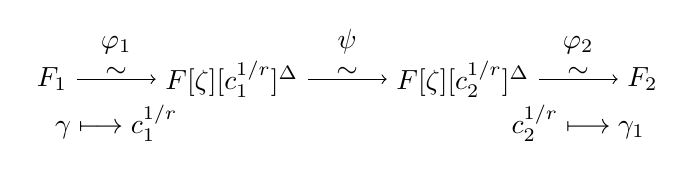
\begin{tikzpicture}
		\node (Fc1) {$F[\zeta][c_1^{1/r}]^\Delta$};
		\node[right = of Fc1] (Fc2) {$F[\zeta][c_2^{1/r}]^\Delta$};
		\node[left = of Fc1] (F1) {$F_1$};
		\node[right = of Fc2] (F2) {$F_2$};
		\draw[->] (F1) edge node[above, inner sep=0.5pt] {$\sim$} node[above = 3mm, inner 
		sep=0.5pt] {$\varphi_1$} node[below = 3mm, inner sep=0.5pt] {$\gamma \longmapsto 
		c_1^{1/r}$} (Fc1);
		\draw[->] (Fc1) edge node[above, inner sep=0.5pt] {$\sim$} node[above = 3mm, inner 
		sep=0.5pt] {$ \psi $} (Fc2);
		\draw[->] (Fc2) edge node[above, inner sep=0.5pt] {$\sim$} node[above = 3mm, inner 
		sep=0.5pt] {$ \varphi_2 $} node[below = 3mm, inner sep=0.5pt] {$c_2^{1/r} \longmapsto 
		\gamma_1$} (F2);
	\end{tikzpicture}
\end{equation*}
of isomorphisms. The following algorithm summarizes the process.
\begin{algorithm}[Lesntra]
	\begin{algorithmic}[1]
		\REQUIRE Field extensions $F_1, F_2$ of $F$ of degree $r$
		\ENSURE An isomorphism $\F_1 \xrightarrow{\sim} F_2$
		\STATE find a generator $c_i$ of $T_{F_i}$ for $i = 1, 2$
		\STATE find isomorphisms $\varphi_i: F_i \xrightarrow{\sim} F[\zeta][c_i^{1/r}]^\Delta$ for 
		$i = 1, 2$
		\STATE compute the integer $j$ such that $c_1 = c_2^j$
		\STATE build the isomorphism $\psi: F[\zeta][c_1^{1/r}]^\Delta \xrightarrow{\sim} 
		F[\zeta][c_2^{1/r}]^\Delta$
		\RETURN $\varphi_2 \circ \psi \circ \varphi_1$
	\end{algorithmic}
\end{algorithm}
A more careful look at the above approach suggests a trade-off between determinism and 
simplicity/practicality. For example, one can replace the ring extension $F[\zeta]$ with the field 
extension $F[\zeta] = F[X] / g(X)$ where $g$ is an irreducible factor of $\Phi_r$. This makes 
things simpler and more practical at the cost of factoring $\Phi_r$ which of course introduces 
indeterminism if one choses to use efficient factoring algorithms.

To find generators for the Teichm\"{u}ller subgroups, Lenstra uses some trace-like formula that 
suggests a version of Hilbert 90 Theorem over rings. Alombert's approach is more or less the same 
as above with more focus on implementation. The idea of the algorithm is to use cyclotomic field 
extensions which in turn allows a more explicit use of Hilbert 90 Theorem to find elements 
$\alpha_1 \in F_1[\zeta]$, and $\alpha_2 \in F_2[\zeta]$. Then $b = \alpha_1^r / \alpha_2^r$ is an 
$r$th power in $F[\zeta]$ from which $b^{1/r}$ can be computed using a root extraction algorithm. 
The isomorphism $F_1[\zeta] \xrightarrow{\sim} F_2[\zeta]$ is then given by $\alpha_1 \mapsto 
b^{1/r}\alpha_2$. Although again no rigorous complexity analysis is presented, one can easily see 
that the dominant cost of this algorithm is solving Hilbert 90 which is done using linear algebra. 
Therefore, the algorithm performs $O(n^{\omega + 1})$ many operations in $F$.


\subsection{Fast variant}
In this section we give an asymptotically faster and more practical version of the above 
algorithms. We replace linear algebra with polynomial arithmetic, and use a trace-like computation 
technique to solve Hilbert 90. 

An overview of the construction is as follows. For simplicity, we assume $q$ is prime in $F = 
\F_q$. Suppose we are given extensions $F_1, F_2$ of $F$ of prime degree $r \ne q$. Let $s$ be 
the order of $q$ in $\mathbb{Z} / r\mathbb{Z}$, and write $q^s - 1 = ur^t$ where $\gcd(r, u) = 1$. 
We first move to cyclotomic field extensions $F[\zeta], F_1[\zeta], F_2[\zeta]$ of degree $s$ over 
$F, F_1, F_2$ respectively, by obtaining an irreducible factor of the $r$th cyclotomic polynomial. 
Then there is a non-$r$-adic residue $\eta \in F[\zeta]$ such that $X^r - \eta$ is irreducible in 
$F[\zeta][X]$. Next we find elements $\alpha_1, \alpha_2$ in $F_1[\zeta], F_2[\zeta]$ to build 
isomorphisms $\varphi_1, \varphi_2$ as in Figure \ref{figure:isom1}. Once we obtain an isomorphism 
$F_1[\zeta] \rightarrow F_2[\zeta]$, we descend it down to an isomorphism $F_1 \rightarrow F_2$. 

Throughout this section we assume the representations
\begin{equation}
\label{equation:rep}
F_1 = F[X] / f(X), \; F[\zeta] = F[Z] / h(Z), \;
F_1[\zeta] = F[X, Z] / (f(X), g(Z))
\end{equation}
where $f(X) \in F[X]$ is an irreducible polynomial of degree $r$, and $h(Z)$ is an irreducible 
factor of the $r$-th cyclotomic polynomial $\Phi_r(Z)$. We also let $x, z = \zeta$ be the residue 
classes of $X, Z$ in these quotients.
\begin{figure}
	\begin{center}
		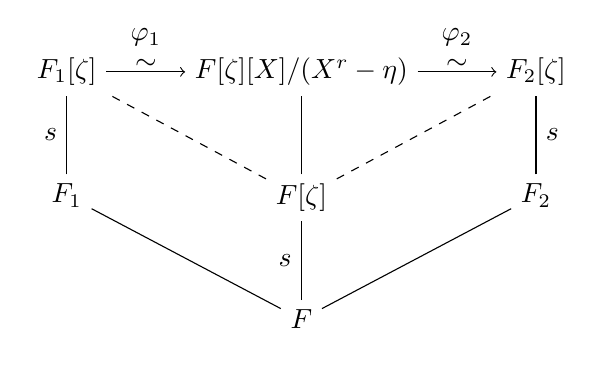
\begin{tikzpicture}
		\node (Fp) {$F$};
		\node[above = of Fp] (Fpz) {$F[\zeta]$};
		\node[above = of Fpz] (Fpzx) {$F[\zeta][X] / (X^r - \eta)$};
		\node[left = of Fpzx] (F1z) {$F_1[\zeta]$};
		\node[right = of Fpzx] (F2z) {$F_2[\zeta]$};
		\node[below = of F1z] (F1) {$F_1$};
		\node[below = of F2z] (F2) {$F_2$};
		\draw (Fp) edge (F1) edge (F2) edge node[left, midway] {$s$} (Fpz)
		(Fpz) edge (Fpzx) edge[dashed] (F1z) edge[dashed] (F2z)
		(F1) edge node[left, midway] {$s$} (F1z)
		(F2) edge node[right, midway] {$s$} (F2z);
		\draw[->] (F1z) edge node[above, inner sep=0.5pt] {$ \sim $} node[above = 3mm, inner 
		sep=0.5pt] {$ \varphi_1 $} (Fpzx);
		\draw[->] (Fpzx) edge node[above, inner sep=0.5pt] {$ \sim $} node[above = 3mm, inner 
		sep=0.5pt] {$ \varphi_2 $} (F2z);
		\end{tikzpicture}
		\caption{Constructing isomorphisms}
		\label{figure:isom1}
	\end{center}
\end{figure}





%///////////////////////////////////////////

\subsubsection{Preliminaries}

As mentioned above, we let $s$ be the order of $q$ in $\mathbb{Z} / r\mathbb{Z}$, and write $q^s - 
1 = ur^t$ where $\gcd(r, u) = 1$. The obvious way constructing isomorphisms $\varphi_1, \varphi_2$ 
in Figure \ref{figure:isom1} is to compute an $r$-th root of $\eta$ in $F_1[\zeta], F_2[\zeta]$. 
But, as a more efficient way, we show how to avoid the costly operation of taking roots in these 
extensions, and skip some detail computations. We first need the following result.
\begin{proposition}
	\label{proposition:semi-trace}
	For an element $a \in F_1[\zeta]$ define 
	\begin{equation}
	\label{equation:semi-trace} 
	\theta_a = a + \zeta^{r - 1}a^{q^s} + \cdots + \zeta^2a^{q^{(r - 2)s}} + \zeta a^{q^{(r - 1)s}}
	\end{equation}
	Then
	\begin{enumerate}
		\item[\normalfont (i)] There is an $a \in F_1[\zeta]$ such that $\theta_a \ne 0$.
		\item[\normalfont (ii)] For a generator $\sigma$ of $\gal(F_1[\zeta] / F[\zeta])$ we have 
		$\sigma(\theta_a) / \theta_a = \zeta$. Also $\theta_a, \theta_a^r$ are non-$r$-adic 
		residues in $F_1[\zeta], F[\zeta]$ respectively.
	\end{enumerate}
\end{proposition}
\begin{proof}
	Let $v = u^{-1} \bmod r$, and let $\gamma \in F_1[\zeta]$ be an $r^t$-th root of $\zeta^{v(r - 
	1)}$. There exists an element $a \in F_1[\zeta]$ such that $\beta = T_{F_1[\zeta] / 
	F[\zeta]}(\gamma a) \ne 0$, and we have 
	\begin{equation}
		\label{equation:trace}
		\begin{aligned}
		\beta 
		& = \gamma a + (\gamma a)^{q^s} + \cdots + (\gamma a)^{q^{(r - 1)s}} \\
		& = \gamma (a + \gamma^{q^s - 1}a^{q^s} + \cdots + \gamma^{q^{(r - 1)s} - 1}a^{q^{(r - 
		1)s}}) \\
		& = \gamma (a + \gamma^{ur^t}a^{q^s} + \cdots + \gamma^{ur^t(q^{(r - 2)s} + \cdots + q^s + 
		1)}a^{q^{(r - 1)s}}) \\
		& = \gamma (a + \zeta^{r - 1}a + \cdots + \zeta a^{q^{(r - 1)s}}) \\
		& = \gamma \theta_a.
		\end{aligned}
	\end{equation}
	This proves (i). To prove (ii), first observe that $\theta_a^{q^s} = \zeta\theta_a$ so that 
	$\sigma(\theta_a) = \zeta\theta_a$ for a generator $\sigma: x \to x^{q^s}$ of $\gal(F_1[\zeta] 
	/ F[\zeta])$. Therefore, we have $\sigma(\theta_a^r) = \theta_a^r$, which means that 
	$\theta_a^r \in F[\zeta]$, and $\theta_a^{ur^t} = \theta_a^{q^s - 1} = \zeta$ which proves 
	that $\theta_a, \theta_a^r$ are non-$r$-adic residues.
\end{proof}
Let $\eta_a = \theta_a^r, \eta_b = \theta_b^r$ for nonzero $\theta_a, \theta_b$ as in Proposition 
\ref{proposition:semi-trace}. Then we can construct isomorphisms $\varphi_1, \varphi_2$ as in the 
following diagram.
\begin{equation}
	\label{equation:iso-chain}
	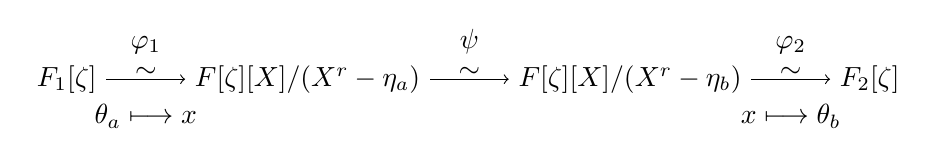
\begin{tikzpicture}
		\node (Fpzxa) {$F[\zeta][X] / (X^r - \eta_a)$};
		\node[right = of Fpzxa] (Fpzxb) {$F[\zeta][X] / (X^r - \eta_b)$};
		\node[left = of Fpzxa] (F1z) {$F_1[\zeta]$};
		\node[right = of Fpzxb] (F2z) {$F_2[\zeta]$};
		\draw[->] (F1z) edge node[above, inner sep=0.5pt] {$ \sim $} node[above = 3mm, inner 
		sep=0.5pt] {$ \varphi_1 $} node[below = 3mm, inner sep=0.5pt] {$\theta_a \longmapsto x$} 
		(Fpzxa);
		\draw[->] (Fpzxa) edge node[above, inner sep=0.5pt] {$ \sim $} node[above = 3mm, inner 
		sep=0.5pt] {$ \psi $} (Fpzxb);
		\draw[->] (Fpzxb) edge node[above, inner sep=0.5pt] {$ \sim $} node[above = 3mm, inner 
		sep=0.5pt] {$ \varphi_2 $} node[below = 3mm, inner sep=0.5pt] {$x \longmapsto \theta_b$} 
		(F2z);
	\end{tikzpicture}
\end{equation}
To complete this isomorphism chain, we need to compute $\psi$. For that we simply compute an $r$-th 
root of $\eta_a$ in $F = F[\zeta][X] / (X^r - \eta_b)$, and construct the 
isomorphism in the obvious way. Note that from (\ref{equation:trace}) we have $\beta_a = 
\gamma_a\theta_a$,  $\beta_b = \gamma_b\theta_b$, and we can choose $\gamma_a, \gamma_b$
such that $\gamma_a^r = \gamma_b^r$. Therefore, 
\[ \eta_a\eta_b^{-1} = \beta_a^r\beta_b^{-r} = (\beta_a\beta_b^{-1})^r = c^r. \] 
So we can construct the isomorphism
\begin{equation*}
	\begin{array}{rrll}
	\psi: & F[\zeta][X] / (X^r - \eta_a) & \longrightarrow & F[\zeta][X] / (X^r - \eta_b) \\
	& x & \longmapsto & cx
	\end{array}
\end{equation*}
by computing an $r$-th root in $F[\zeta]$.




%///////////////////////////////////////////

\subsubsection{Computing $\theta_a$}

Let $a \in F_1[\zeta]$. To compute $\theta_a$, we use a binary powering scheme similar to the one 
in \cite{doliskanischost2011}. Assuming the representations (\ref{equation:rep}) we let 
\[
\xi_i = x^{q^{is}}, \quad
\delta_i = a + z^{r - 1}a^{q^s} + \cdots + z^2a^{q^{(i - 1)s}} + z^{r - i + 1} a^{q^{(i - 1)s}}.
\]
Then we have the following relations:
\[\xi_1 = x^{q^s}, \quad \delta_1 = a, \]
\[
\xi_i =
\begin{cases}
\xi_{i / 2}^{q^{is / 2}} & \text{if $i$ is even}  \\
\xi_{i - 1}^{q^s} & \text{if $i$ is odd,}
\end{cases} \quad
\delta_i=
\begin{cases}
z^{r - i / 2}\delta_{i / 2}^{q^{is / 2}} + \delta_{i / 2} & \text{if $i$ is even} \\
z^{r - 1}\delta_{i - 1}^{q^s} + \delta_1 & \text{if $i$ is odd}
\end{cases}
\]
Assuming $\xi_i = x^{q^{is}}$ is already known, $\delta_i$ can be computed using the following 
algorithm.

\begin{algorithm}
	[XiDelta$(i, \xi_1,\delta_1)$]
	\label{algorithm:xidelta}
	\begin{algorithmic}[1]
		\REQUIRE a positive integer $i$, $\xi_1 = x^{q^s}$, $\delta_1 = a$
		\ENSURE $\xi_i$, $\delta_i$
		\IF {$i=1$} 
		\RETURN $\xi_1$, $\delta_1$
		\ENDIF
		\STATE $j \leftarrow \lfloor i/2\rfloor$
		\STATE $\xi_{j}, \delta_j \leftarrow {\rm XiDelta}(j,\xi_1,\delta_1)$ 
		\STATE\label{step:xi} $\xi_{2j} \leftarrow \xi_j(\xi_j)$
		\STATE\label{step:delta} $\delta_{2j} \leftarrow z^{r - j}\delta_j(\xi_j) + \delta_j$
		\IF {$i$ is even} 
		\RETURN $\xi_{2j}$, $\delta_{2j}$
		\ENDIF
		\STATE $\xi_i \leftarrow \xi_{2j}(\xi_1)$
		\STATE $\delta_i \leftarrow z^{r - 1}\delta_j(\xi_1) + \delta_1$
		\RETURN $\xi_i$, $\delta_i$
	\end{algorithmic}
\end{algorithm}

\begin{proposition}
	\label{proposition:XiDelta}
	Finding a nonzero $\theta_a$ for random $a \in F_1[\zeta]$ takes \[O(s\CC(r)\log(r) + 
	\MM(r)\log(q))\] operations in $F$.
\end{proposition}
\begin{proof}
	To compute the initial value $\xi_1 = x^{q^s}$ we first compute $x^q$, and then do $\log(s)$ 
	modular compositions at a total cost of $O(\MM(r)\log(q) + C(r)\log(s))$ operations in $F$. 
	Then $\theta_a = \delta_r$ is computed using Algorithm \ref{algorithm:xidelta}: the complexity 
	of the algorithm is dominated by steps \ref{step:xi}, \ref{step:delta}. The former is a
	modular composition in $F[X]$ which takes $C(r)$ operations in $F$. For the later suppose 
	$\delta_j = \delta_{j,0}(x) + \delta_{j,1}(x)z + \cdots + \delta_{j,s - 1}(x)z^{s - 1}$. Then   
	\[ \delta_j(\xi_j) = \sum_{i = 0}^{s - 1}\delta_{ij}(\xi_j)z^i, \] which is done using 
	$O(s\CC(r))$ operations in $F$. Accounting for a recursion depth of $\log(r)$, the running 
	time of the algorithm is then $O(s\CC(r)\log(r))$ operations in $F$. All in all, we get the 
	claimed 
	complexity.
\end{proof}
The above running time for computing $\theta_a$ is only acceptable for small $s$. More precisely, 
if we take $\CC(r) = O(r^{(1 + \omega) / 2})$ then the running time becomes quadratic if $s \approx 
r^{(3 - \omega) / 2}$. We call $s$ small if $s < r^{(3 - \omega) / 2}$, and large otherwise. To 
keep the complexity at most quadratic for all $s$, we proceed as follows. We know that 
$T_{F_1[\zeta] / F[\zeta]}(\gamma x^\ell) \ne 0$ for at least one $1 \le \ell \le r - 1$, otherwise 
$T_{F_1[\zeta] / F[\zeta]}(\gamma a) = 0$ for all $a \in F_1[\zeta]$ by linearity. Therefore, the 
linear map 
\[
\begin{array}{rrll}
	T_{F_1[\zeta] / F[\zeta]}\vert_{F_1}: & F_1 & \longrightarrow & F[\zeta] \\
	& d(x) & \longmapsto & T_{F_1[\zeta] / F[\zeta]}(\gamma d(x))
\end{array}
\]
is not identically zero. This implies that we need to try at most $O(1)$ random $d(x) \in F_1$ to 
obtain a nonzero
\[ \theta_{d(x)} = d(x) + \zeta^{r - 1}d(x)^{q^s} + \cdots + \zeta^2d(x)^{q^{(r - 2)s}} + \zeta 
d(x)^{q^{(r - 1)s}}. \]
The sequence $d(x), d(x)^{q^s}, \dots, d(x)^{q^{(r - 1)s}}$ in $F_1$ can be computed by Algorithm 
3.1 in \cite{von1992computing} using $O(\MM(r^2)\log(r))$ operations in $F$. Therefore, we have 
proved the following,
\begin{proposition}
	\label{proposition:XiDelta-updated}
	Finding a nonzero $\theta_a$ for random $a \in F_1[\zeta]$ takes
	\begin{itemize}
		\item $O(s\CC(r)\log(r) + \MM(r)\log(q))$ operations in $F$ for small $s$, or
		\item $O(\MM(r^2)\log(r) + \MM(r)\log(q))$ operations in $F$ for large $s$.
	\end{itemize}
\end{proposition}



%///////////////////////////////////////////

\subsubsection{Computing $r$-th roots in $F[\zeta]$}
\label{subsection:rth-root-fpz}

Let $a \in F[\zeta]$ be an $r$-th power. To compute an $r$-th root of $a$ we factor the 
polynomial $X^r - a$ using the Equal Degree Factorization algorithm given in 
\cite{kaltofen+shoup97}.
\begin{algorithm}
	[Root Finding]
	\label{algorithm:edf}
	\begin{algorithmic}[1]
		\REQUIRE a square-free polynomial $f \in F[\zeta][x]$ of degree $n$ with linear factors
		\ENSURE a single factor of $f$
		\IF {$\deg f = 1$}
		\RETURN $f$
		\ENDIF
		\STATE Pick a random element $\alpha \in \mathbb{A}_f = F[\zeta][x]/f$
		\STATE\label{step:edf-trace} Compute the following trace in $\mathbb{A}_f$
		\[ \beta = \alpha + \alpha^q + \alpha^{q^2} + \cdots + \alpha^{q^{s - 1}} \]
		\STATE $\gamma \leftarrow \beta^{(q - 1) / 2}$
		\STATE $g \leftarrow \gamma \bmod f$, $g_1 \leftarrow \gcd(g, f)$, $g_2 \leftarrow \gcd(1 + 
		g, f)$, $g_3 \leftarrow f/(g_1g_2)$
		\STATE Recursively factor one of $g_1, g_2, g_3$ that is non-constant
	\end{algorithmic}
\end{algorithm}
The dominant cost of the algorithm comes from Step \ref{step:edf-trace}, which is done as follows. 
Let
\[ \beta_i = \alpha^q + \alpha^{q^2} + \cdots + \alpha^{q^i}, \quad \xi_i = x^{q^i}, \quad \zeta_i 
= z^{q^i}. \]
Then we have $\beta_1 = \alpha^q$, $\xi_1 = x^q$, $\zeta_1 = z^q$, and
\[
\beta_j = 
\begin{cases}
	\beta_{j / 2} + \beta_{j / 2}^{q^{j / 2}} & j \text{ even} \\
	\beta_1 + \beta_{j - 1}^q & j \text{ odd}
\end{cases}, \quad
\xi_j = 
\begin{cases}
	\xi_{j / 2}^{q^{j / 2}} & j \text{ even} \\
	\xi_{j - 1}^q & j \text{ odd}
\end{cases}, \quad
\zeta_j = 
\begin{cases}
	\zeta_{j / 2}^{q^{j / 2}} & j \text{ even} \\
	\zeta_{j - 1}^q & j \text{ odd}
\end{cases}
\]
For a positive integer $j$ we have
\begin{equation}
	\label{equation:betaj}
	\beta_j^{q^j} = \left( \sum_{l = 0}^{n - 1}c_l(z)x^l \right)^{q^j} = \sum_{l = 0}^{n - 
	1}c_l(z^{q^j})(x^{q^j})^l = \sum_{l = 0}^{n - 1}c_l(\zeta_j)\xi_j^l.
\end{equation}
Therefore we have a recursive algorithm for computing $\beta = \beta_{s - 1}$. Let us analyze the 
complexity of the algorithm. First note that we always have $z^r = 1, x^r = a$. This makes it 
possible to keep the identities simple and do the reductions at the end of each step. For example 
$x^q = a^{\lfloor q / r\rfloor}x^{q \bmod r}$ which can be computed using $O(\MM(s)\log(q))$
operations in $F$. At step $j$ of the recursion we have the following costs in $F$:
\begin{itemize}
	\item $O(\MM(r) + \MM(s)\log(r))$ for computing $x^{q^j}$, and computing $z^{q^j}$ is free.
	\item If $s$ is small we can first reduce $z^{q^j \bmod r}$ modulo $g(Z)$, and then do $n$ 
	modular compositions at a total cost
	of $O(\MM(r) + n\CC(s))$. But if $s$ is large we can reduce $c_l(z^{q^j \bmod r})$ modulo 
	$g(Z)$ for all $0 \le l < n$ at a total cost of $O(n\MM(r))$.
	\item $O(n\MM(s))$ for evaluating $\beta_j$ at $x^{q^j}$ using Horner's method.
	\item $O(\MM(r)\MM(s))$ for reducing (\ref{equation:betaj}) modulo $f$.
\end{itemize}
The depth of the recursion is $\log(s)$, hence $\beta$ can be computed in
\begin{itemize}
	\item $O(\MM(s)\log(q) + n\CC(s)\log(s) + \MM(r)\MM(s)\log(s))$ operations in $F$ for small 
	$s$, or
	\item $O(\MM(s)\log(q) + n\MM(r)\log(s) + \MM(r)\MM(s)\log(s))$ operations in $F$ for large 
	$s$.
\end{itemize} 
Finally since the depth of the recursion in Algorithm \ref{algorithm:edf} is $\log(r)$, we have the 
following.
\begin{proposition}
	\label{proposition:root-fpz}
	The total cost of root finding in $F[\zeta]$ is
	\begin{itemize}
		\item $O(\MM(s)\log(q)\log(r) + r\CC(s)\log(s) + \MM(r)\MM(s)\log(s)\log(r))$\\ operations 
		in $F$ for small $s$, or
		\item $O(\MM(s)\log(q)\log(r) + r\MM(r)\log(s) + \MM(r)\MM(s)\log(s)\log(r))$\\ operations 
		in $F$ for large $s$.
	\end{itemize}
\end{proposition}





%///////////////////////////////////////////

\subsubsection{Computing the isomorphism $F_1 \rightarrow F_2$}

In this section, we analyze the computational cost of building an isomorphism $\varphi: F_1 
\rightarrow F_2$. We first construct the isomorphism $\varphi_2 \circ \psi \circ \varphi_1 : 
F_1[\zeta] \rightarrow F_2[\zeta]$ as in (\ref{equation:iso-chain}), and then descend back to the 
desired fields. The following algorithm builds the above chain of isomorphism based on the 
observations at the start of the section. 
\begin{algorithm}
	[Isomorphism ${F_1[\zeta] \rightarrow F_2[\zeta]}$]
	\label{algorithm:ext-iso}
	\begin{algorithmic}[1]
		\REQUIRE degree $r$ extensions $F_1, F_2$ of $F$
		\ENSURE an isomorphism $F_1[\zeta] \rightarrow F_2[\zeta]$
		\STATE\label{step:factor-cyclo} factor the cyclotomic polynomial $\Phi_r(Z)$ over $F$ to 
		build extensions $F[\zeta],	F_1[\zeta], F_2[\zeta]$
		\REPEAT
		\STATE choose a random $a \in F_1[\zeta]$
		\STATE compute $\theta_a$ using Algorithm \ref{algorithm:xidelta}
		\UNTIL {$\theta_a \ne 0$}
		\REPEAT
		\STATE choose a random $b \in F_2[\zeta]$
		\STATE compute $\theta_b$ using Algorithm \ref{algorithm:xidelta}
		\UNTIL {$\theta_b \ne 0$}
		\STATE\label{step:gamma-pow} $\eta_a \leftarrow \theta_a^r$ , $\eta_b \leftarrow \theta_b^r$
		\STATE\label{step:psi} construct the isomorphism $\psi$ as in (\ref{equation:iso-chain})
		\STATE construct $F_1[\zeta] \rightarrow F_2[\zeta]$ as in (\ref{equation:iso-chain})
	\end{algorithmic}
\end{algorithm}
\begin{proposition}
	Algorithm \ref{algorithm:ext-iso} computes the isomorphism $F_1[\zeta] \rightarrow F_2[\zeta]$ 
	using
	\begin{itemize}
		\item $O(s\CC(r)\log(r) + \MM(r)\log(q) + \MM(s)\log(q)\log(r))$\\ operations in $F$ for 
		small $s$, or
		\item $O(\MM(r)\log(q) + \MM(s)\log(q)\log(r) + \MM(r^2)\log(r) +  
		\MM(s)\MM(r)\log(s)\log(r))$\\ 
		operations in $F$ for large $s$.
	\end{itemize}
\end{proposition}
\begin{proof}
	By \cite[Theorem 9]{shoup94} Step \ref{step:factor-cyclo} takes $O(r\log^2(r) + 
	r\log(r)\log(q))$ operations in $F$. The running time of the two repeat...until loops is 
	given by Proposition \ref{proposition:XiDelta-updated}. Step \ref{step:gamma-pow}
	is done using $O(\MM(s)\MM(r)\log(r))$ operations in $F$. The running time of Step 
	\ref{step:psi} is given by Proposition \ref{proposition:root-fpz}. Adding all these up proves 
	the proposition.
\end{proof}
So, now we have an isomorphism $\phi: F_1[\zeta] \rightarrow F_2[\zeta]$ that sends $\theta_a$ to 
some $h(z, x) \in F_2[\zeta]$. To construct the isomorphism $\varphi: F_1 \rightarrow F_2$ we the 
technique in \cite{Allombert02}. Let 
\[ \theta_a = \sum_{i = 0}^{s - 1}f_i(x)z^i, \quad\text{and}\quad z^s = (v(z)  \bmod g(z)) = 
\sum_{i = 0}^{s - 1}v_iz^i. \] 
Then since $\theta_a^{q^s} = z\theta_a$ we have
\[ \sum_{i = 0}^{s - 1}f_i(x)^{p^s}z^i = f_{s - 1}(x)v(z) + f_0(x)z + \cdots + f_{s - 2}(x)z^{s - 
1}.\]
After rearranging the terms in the right hand side, this gives us the identities
\[
\begin{array}{ccc}
	f_0(x)^{p^s} & = & v_0f_{s - 1}(x) \\
	f_1(x)^{p^s} & = & f_0(x) + v_1f_{s - 1}(x) \\
	\vdots & \vdots & \vdots \\
	f_{s - 1}(x)^{p^s} & = & f_{s - 2}(x) + v_{s - 1}f_{s - 1}(x)
\end{array} 
\]
form which we see that $f_i(x) \in F(f_0(x)) \subseteq F_1$ for all $i$. We prove $F(f_0) = 
F_1$. Let $\sigma \in \gal(F_1(z) / F)$ be a generator, and let $j \le r$ be the smallest 
integer such that $\sigma^jf_0 = f_0$. Then $\sigma^{js}\theta_a = \theta_a$, but $\theta_a$ is not 
contained in any proper subfield; so $j = r$. Let $h_0$ be the constant term of $h(z, x)$. Then we 
similarly have $F_2 = F(h_0)$. This gives us an isomorphism
\[
\begin{array}{rlll}
	\phi: & F_1 & \longrightarrow & F_2 \\
	& f_0 & \longmapsto & h_0
\end{array}
\]
from which we can get an isomorphism
\[
\begin{array}{rlll}
	\phi: & F_1 & \longrightarrow & F_2 \\
	& x & \longmapsto & a(x)
\end{array}
\]
using transposed modular composition.

\subsubsection{The Artin-Schreier case}
\label{sec:artin-schreier-case}

\todo{We have to write at least a few paragraphs on how to handle this case.}


%%%%%%%%%%%%%%%%%%%%%%%%%%%%%%%%%%
\section{Rains' algorithm}

We now move on to a family of algorithms based on the theory of
algebraic groups. The simplest of these algorithms is Pinch's
cyclotomic algorithm~\cite{Pinch}. The idea is very simple: given $r$,
select a integer $\ell$ such that $[\F_q[\mu_\ell]:\F_q]=r$, where
$\mu_\ell$ is the group of $\ell$-th roots of unity.  Then, any
embedding $k\to K$ takes $\mu_\ell\subset k^\ast$ to $\mu_\ell\subset
K^\ast$, and the minimal polynomial of any primitive $\ell$-th root of
unity has degree exactly $r$.

Pinch's algorithm is very effective when $r=\euler(\ell)$. Indeed in
this case the $\ell$-th cyclotomic polynomial $\Phi_\ell$ is
irreducible over $\F_q$, and its roots form a unique orbit under the
action of the absolute Galois group of $\F_q$. Thus we can take any
primitive $\ell$-th roots of unity $\alpha\in k$ and $\beta\in K$ to
describe the embedding.

In the general case, however, the roots of $\Phi_\ell$ are partitioned
in $\euler(\ell)/r$ orbits, thus for two randomly chosen $\ell$-th
roots of unity $\zeta_1\in k$ and $\zeta_2\in K$, we can only say that
there exists an exponent $e$ such that
\begin{equation*}
  \alpha = \zeta_1 \mapsto \zeta_2^e = \beta
\end{equation*}
defines a valid embedding. Pinch's algorithm tests all possible
exponents $e$, until a suitable one is found. To test for the validity
of a given $e$, it applies the embedding $\phi:\zeta_1\mapsto\zeta_2$
to the class of $X$ in $k$, and verfies that its image is a root of
$f$ in $K$ (see Part~\ref{part:eval} for details on embedding
evaluation).

The trial-and-error nature of Pinch's algorithm makes it impractical,
except for rare favorable cases where a \emph{small} $\ell$ such that
$r=\euler(\ell)$ can be found. One possible workaround, suggested by
Pinch himself, is to replace the group of roots of unity with a group
of torsion points of a well chosen elliptic curve. We analyze this
idea in greater detail in Section~\ref{sec:rains-elliptic}.

This section is devoted to a different way of improving Pinch's
algorithm, imagined by Rains~\cite{rains2008}, and implemented in the
Magma computer algebra system~\cite{MAGMA}. Rains' original preprint
went unpublished\footnote{The only publicly available source for
  Rains' algorithm is Magma's source code (file
  \texttt{package/Ring/FldFin/embed.m}, since v2.14).}, thus we
describe his algorithm in detail for completeness. Rains' technical
contribution is twofold: first he replaces roots of unity with
Gaussian periods to avoid trial-and-error, second he moves to slightly
larger extension fields to insure the existence of a small $\ell$ as
above.

\subsection{Uniquely defined orbits from Gaussian periods}

For the rest of the section, we are going to assume that $q$ is
prime. The case where $q$ is a higher power of a prime is discussed in
Note~\ref{note:rains-non-prime}.

Suppose that we have an $\ell$, coprime with $q$, such that
$[\F_q[\mu_\ell]:\F_q]=r$, then the cyclotomic polynomial $\Phi_\ell$
factors over $\F_q$ into $\euler(\ell)/r$ distinct factors of degree
$r$. Pinch's method, by choosing random roots of $\Phi_\ell$ in $k$
and $K$, randomly selects one of these factors as minimal polynomial.

By combining the roots of $\Phi_\ell$ into Gaussian periods, Rains'
method uniquely selects a minimal polynomial of degree $r$. The
construction is best understood by looking at the Galois groups of
cyclotomic fields. It is well known that the Galois group of
$\Q[\mu_\ell]/\Q$ is canonically isomorphic to $(\Z/\ell\Z)^\ast$ via
the mapping
\begin{equation*}
  \begin{aligned}
    (\Z/\ell\Z)^\ast &\to \gal(\Q[\mu_\ell]/\Q),\\
    e &\mapsto (\sigma_e : \zeta_\ell\mapsto\zeta_\ell^e),
  \end{aligned}
\end{equation*}
where $\sigma_e$ is the map sending any $\ell$-th root of unity to its
$e$-th power, extended by linearity to all of $\Q[\mu_\ell]$. Gaussian
periods are defined as traces of generators of $\mu_\ell$ down to a
subfield of $\Q[\mu_\ell]$.

\begin{definition}
  Let $S$ be a subgroup of $(\Z/\ell\Z)^\ast$, and let $L$ be the
  subfield of $\Q[\mu_\ell]$ fixed by $S$. For any generator
  $\zeta_\ell$ of $\mu_\ell$, define the Gaussian period
  $\eta(\zeta_\ell)$ as
  \begin{equation}
    \eta(\zeta_\ell) = \trace_{\Q[\mu_\ell]/L} \zeta_\ell = \sum_{\sigma\in S}{\zeta_\ell^{\sigma}}.
  \end{equation}
\end{definition}

By hypothesis, the prime $q$ factors as a product of $\euler(\ell)/r$
distinct primes ideals in $\Z[\mu_\ell]$. Let $\mathfrak{q}$ be one
such prime ideal, then $\F_q[\mu_\ell]$ is isomorphic to the residue
field $\Z[\mu_\ell]/\mathfrak{q}$, and we can identify (canonically)
the Galois group $\gal(\F_q[\mu_\ell]/\F_q)$ with the subgroup
$\langle q\rangle\subset(\Z/\ell\Z)^\ast$.

Now, suppose there is a group $S$ such that
$(\Z/\ell\Z)^\ast=S\times\langle q\rangle$, let $L$ be the field fixed
by $S$, and let $\mathcal{O}_L$ be its ring of integers. Then, the
Galois group of $L/\Q$ is also canonically identified with $\langle
q\rangle\subset(\Z/\ell\Z)^\ast$, the prime $q$ is inert in $L$, and
$\mathcal{O}_L/q\mathcal{O}_L$ is isomorphic to
$\F_q[\mu_\ell]$. While the identification of $\F_q[\mu_\ell]$ with
$\Z[\mu_\ell]/\mathfrak{q}$ depended on the choice of the prime
$\mathfrak{q}$, taking the trace down to $L$ and then reducing modulo
$q$ is independent of such choice, we obtain thus a canonical
identification between $\mathcal{O}_L/q\mathcal{O}_L$ and
$\F_q[\mu_\ell]$. The situation is summarized in the following
diagram:
\begin{equation*}
  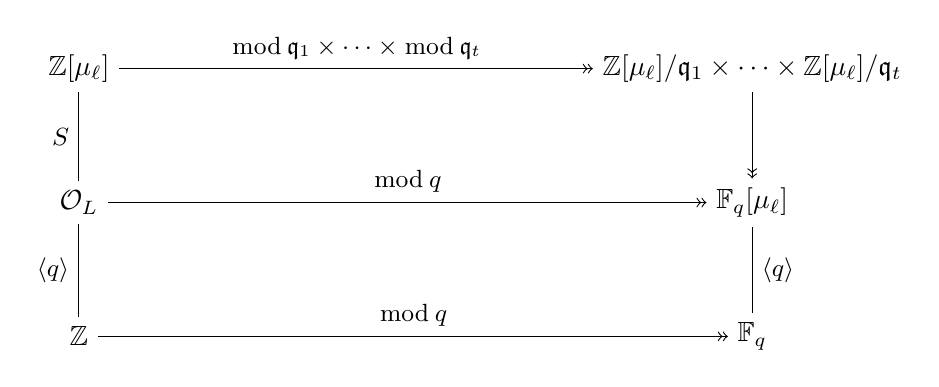
\begin{tikzpicture}[node distance=1.7cm]
    \node (Q) {$\Z$};
    \node[above of=Q] (L) {$\mathcal{O}_L$};
    \node[above of=L] (Qm) {$\Z[\mu_\ell]$};
    \node[right=8cm of Q] (Fp) {$\F_q$};
    \node[above of=Fp] (Fpm) {$\F_q[\mu_\ell]$};
    \node[above of=Fpm] (Prod) {$\Z[\mu_\ell]/\mathfrak{q}_1\times\cdots\times\Z[\mu_\ell]/\mathfrak{q}_t$};
    \draw 
    (Q) edge node[left] {\small $\langle q\rangle$} (L)
    (L) edge node[left] {\small $S$} (Qm)
    (Fp) edge node[right] {\small $\langle q\rangle$} (Fpm); 
    \draw[->>] 
    (Q) edge node[above] {\small $\bmod\, q$} (Fp)
    (L) edge node[above] {\small $\bmod\, q$} (Fpm)
    (Qm) edge node[above] {\small $\bmod\, \mathfrak{q}_1\times\cdots\times\bmod\,\mathfrak{q}_t$} (Prod)
    (Prod) edge node[right] {} (Fpm);
  \end{tikzpicture}
\end{equation*}

We can now extend the definition of Gaussian period to finite fields.

\begin{definition}
  Suppose that there is a subgroup $S\subset(\Z/\ell\Z)^\ast$ such
  that $(\Z/\ell\Z)^\ast=S\times\langle q\rangle$. For any generator
  $\zeta_\ell$ of $\mu_\ell$ in $\F_q[\mu_\ell]$, define the Gaussian
  period $\eta_q(\zeta_\ell)$ as
  \begin{equation}
    \eta_q(\zeta_\ell) = \sum_{\sigma\in S}{\zeta_\ell^{\sigma}}.
  \end{equation}
\end{definition}

\begin{lemma}
  \label{th:gaussian}
  Let $\ell$ be a squarefree integer such that $(\Z/\ell\Z)^\ast = S
  \times \langle q\rangle$ for some $S$.  The periods
  $\eta_q(\zeta_\ell^\sigma)$ for $\sigma$ running through $\langle
  q\rangle$ form a normal basis of $\F_q[\mu_\ell]$ over $\F_q$,
  independent of the choice of $\zeta_\ell$.
\end{lemma}
\begin{proof}
  See~\cite[Main Theorem]{feisel1999normal}.
\end{proof}

In what follows we are going to write $\eta(\zeta_\ell)$ when $q$ is
clear from the context.

\begin{example} 
  Consider the extension $\F_8/\F_2$ of degree $3$, which is generated
  by the $7$-th roots of unity. We have a decomposition
  $(\Z/7\Z)^\ast=\langle 2\rangle\times\langle-1\rangle$, and the
  cyclotomic polynomial factors as
  \begin{equation}
    \Phi_7(x) = (x^3 + x + 1) (x^3 + x^2 + 1).
  \end{equation}
  For any root $\zeta_7$, we define the period
  \begin{equation}
    \eta_2(\zeta_7) = \zeta_7+\zeta_7^{-1}.
  \end{equation}
  The three periods $\eta_2(\zeta_7)$, $\eta_2(\zeta_7)^2$ and
  $\eta_2(\zeta_7)^4$ are all roots of the polynomial $x^3+x^2+1$ and
  form a normal basis of $\F_8/\F_2$.
\end{example}

\subsection{Rains' cyclotomic algorithm}

The bottom-line of Rains' algorithm follows immediately from the
previous section: given $k$, $K$ and $r$,
\begin{enumerate}
\item find a \emph{small} $\ell$ satisfying the conditions of
  Lemma~\ref{th:gaussian} with $[\F_q[\mu_\ell]:\F_q]=r$;
\item take random $\ell$-th roots of unity $\zeta_\ell\in k$ and
  $\zeta_\ell'\in K$;
\item return the Gaussian periods $\alpha=\eta(\zeta_\ell)$ and
  $\beta=\eta(\zeta_\ell')$.
\end{enumerate}

The problem with this algorithm is the vaguely defined
\emph{smallness} requirement on $\ell$. Indeed the conditions of
Lemma~\ref{th:gaussian} imply that $\ell$ divides $\Phi_r(q)$, thus in
the worst case $\ell$ can be as large as $O(q^{\euler(r)})$, which
yields an algorithm of exponential complexity in the field size.

To circumvent this problem, Rains allows the algorithm to work in
small auxiliary extensions of $k$ and $K$, and then descend the
results to $k$ and $K$ via a field trace. In other words, Rains'
algorithm looks for $\ell$ such that $[\F_q[\mu_\ell]:\F_q]=rs$ for
some small $s$. We summarize this method in
Algorithm~\ref{algorithm:rains-cyclo}; we only give the procedure for
the smaller field $k$, the procedure for the larger field $K$ being
identical.

\begin{algorithm}[Rains' cyclotomic algorithm]
  \label{algorithm:rains-cyclo}
  \begin{algorithmic}[1]
    \REQUIRE A field extension $k/\F_q$ of degree $m$, a prime power
    $r|m$, a prime $\ell$ such that
    \begin{itemize}
    \item $(\Z/\ell\Z)^\ast = S \times \langle q\rangle$ for some $S$,
    \item $\#\langle q\rangle = rs$ for some integer $s$.
    \end{itemize}
    \ENSURE A normal generator of $\F_{q^r}\subset k$ over $\F_q$,
    with a uniquely defined Galois orbit.
    
    \STATE Construct the smallest field extension $k'/k$
    containing $\F_{q^{rs}}$; 
    \REPEAT
    \STATE Compute $\zeta = \theta^{(\#k'-1)/\ell}$ for a random $\theta\in k'$
    \UNTIL $\zeta$ is a primitive $\ell$-th root of unity;
    \STATE\label{algorithm:rains-cyclo:period} Compute $\eta(\zeta) = \sum_{\sigma\in S}\zeta^\sigma$;
    \RETURN\label{algorithm:rains-cyclo:trace} $\alpha = \trace_{\F_{q^{rs}}/\F_{q^r}}\eta(\zeta) = \sum_{i=0}^{s-1}\eta(\zeta)^{q^{ri}}$.
  \end{algorithmic}
\end{algorithm}

\begin{proposition}
  Algorithm~\ref{algorithm:rains-cyclo} is correct. On input
  $m,q,r,\ell,s$ it computes its output using $O(\MM(ms)(ms\log q +
  (\ell\log\ell)/r))$ operations in $\F_q$, or $\tildO(m^2s^2\log q)$
  assuming $\ell\in o(mrs)$.
\end{proposition}
\begin{proof}
  By construction $k'$ contains a subfield isomorphic to $\F_{q^{rs}}$
  and to $\F_q[\mu_\ell]$. By Lemma~\ref{th:gaussian} $\eta(\zeta)$ is
  a normal generator of $\F_{q^{rs}}$, and
  by~\cite[Prop.~5.2.3.1]{mullen2013handbook} is a normal generator of
  $\F_{q^r}\subset k$.

  In the worst case $[k':k]=s$. Using the techniques
  in~\cite{couveignes+lercier11,DeDoSc13,DeFeo:2014:FAA:2608628.2608672},
  $k'$ can be constructed, and elements can be moved between $k$ and
  $k'$ using $O(\MM(ms))$ operations in $\F_q$ \todo{This is very
    optimistic, esp. if $s$ is not coprime to $m$}.

  The root of unity $\zeta$ is obtained after $O(1)$ tries on average,
  at a cost of $O(\MM(ms)ms\log q)$ operations each.
  Steps~\ref{algorithm:rains-cyclo:period}
  and~\ref{algorithm:rains-cyclo:trace} can be performed at once by
  observing that
  \[\alpha = \sum_{i=0}^{s-1}\eta(\zeta^{q^{ri}})= \sum_{i=0}^{s-1}\sum_{\sigma\in S}\zeta^{q^{ri}\sigma}.\]
  By reducing $q^{ri}\sigma$ modulo $\ell$, we can compute this sum at
  the cost of $\euler(\ell)/r$ exponentiations of degree at most
  $\ell$ in $k'$, for a total cost of $O((\MM(ms)\ell\log\ell)/r)$.
\end{proof}

This concludes the presentation of Rains' algorithm. However, we are
still left with a problem: how to find $\ell$ satisfying the
conditions of the algorithm, and what bounds can be given on it. These
questions will be analyzed in Section~\ref{sec:selection}.

\begin{remark}
  Various practical optimizations are possible for Rains'
  algorithm. We list here some of them.
  \begin{itemize}
  \item If $s$ cannot be chosen so that $k'=k$, then it is interesting
    to take $s$ coprime with $m$. In this case, the extension $k$' can
    be built using a polynomial with coefficients in $\F_q$ rather
    than $k$, and a lookup table of irreducible polynomials can be
    established for small $s$.
  \item Different prime powers $r_1,r_2,\dots$ can be treated
    simultaneously in some cases. We come back to this in
    Section~\ref{sec:selection}.
  \item In some cases, the trace in the final step can be computed
    more efficiently by exploiting the fact that it is a linear form,
    as per~\cite{todo}.
  \end{itemize}
\end{remark}

\begin{note}
  \label{note:rains-non-prime}
  Rains' algorithm is easily extended to a non-prime field $\F_q$, as
  long as $q=p^d$ with $\gcd(d,r)=1$. In this case, indeed, any
  generator of $\F_{p^r}$ over $\F_p$ is also a generator of
  $\F_{q^r}$ over $\F_q$. The algorithm is unchanged, except for the
  additional requirement that $\gcd(\euler(\ell),d)=1$, which ensures
  that the Gaussian periods indeed generate $\F_{p^r}$.

  However, when $\gcd(d,r)\ne 1$, it is impossible to have
  $(\Z/\ell\Z)^\ast=S\times\langle q\rangle$, so Rains' algorithm
  simply cannot be applied to this case. In the next section we are
  going to present a variant that does not suffer from this problem.
\end{note}


%%%%%%%%%%%%%%%%%%%%%%%%%%%%%%%%%%

\section{Elliptic Rains' algorithm}
\label{sec:rains-elliptic}

In \cite{Pinch}, Pinch already proposed to use the torsion points of an elliptic
curve in place of the roots of unity. Rains also mentionned this possiblity, 
but judged that as far as he could see, it would not bring significant 
improvements.
 
In practice the use of auxiliary extensions in the cyclotomic method costs a
lot of ressources. We will see that, contrary to Rains' belief, in the cases 
where an auxiliary extention is necessary, the elliptic variant is actually more 
competitive.

In the next sections, we will first introduce the \emph{elliptic periods} which 
similar to the Gaussian periods will form a normal basis of $\F_q^r$, then we will 
describe the algorithm itself, namely how to pick the right elliptic curve and
how to compute the \emph{elliptic periods}.
 
\subsection{Uniquely defined orbits from elliptic periods}

In the previous section, the group used to compute our generating elements was
the group of primitive roots of unity. For this variant, we use the group of
torsion point of a certain elliptic curve. There are polynomials that encode 
torsion points, they are called divisions polynomial. More precisely, for
all integers $\ell$, the roots of the division polynomial $\psi_\ell$ are exactly the 
abscissas of the points in $E[\ell]$. Since $E[\ell]$ is either isomorphic to 
$\Z/\ell\Z\times\Z/\ell\Z$, $\Z/\ell\Z$ or $0$, we have the following
\begin{equation}
\deg(\psi_\ell) = \begin{cases}
   \tfrac{(\ell^2-1)}{2} &\text{ if }E[\ell]\simeq\Z/\ell\Z\times\Z/\ell\Z\\
   \tfrac{(\ell-1)}{2} &\text{ if }E[\ell]\simeq\Z/\ell\Z\\
   0 &\text{ if } E[\ell]\simeq\lbrace{0}\rbrace\\
\end{cases}
\end{equation}
As for the roots of unity in the cyclotomic section, the goal will be to sum
specific roots of a division polynomial to generate elements with a common orbit
under the action of a certain Galois group. For our algorithm to work, we will 
need the degree of the division polynomial to be equal to $(\ell^2 - 1)/2$,
\emph{i.e.} we need the \emph{Elkies primes}.

\begin{definition}
Let $E/\F_q$ be an elliptic curve, let $\ell$ be a prime, we say that $\ell$
is an Elkies prime for $E$ if the charateristic polynomial of its Frobenius
$\pi_q : (X, Y, Z) \to (X^q, Y^q, Z^q)$ splits in $\Z/\ell\Z$, in other words
\begin{equation}
X^2-tX+q=(X-\lambda)(X-\mu)\bmod\ell
\end{equation}
for $\lambda,\mu\in\Z/\ell\Z$ and $t$ the trace of the Frobenius $\pi_q$ such that 
$\#E(\F_q)=q+1-t$.
\end{definition}

If $\ell$ is an Elkies prime for $E$, then the restriction of $\pi_q$ on
$E[\ell]$ splits in two eigenspaces. Those are associated to the eigenvalues,
roots of the charateristic polynomial of the Frobenius in $(\Z/\ell\Z)$. 
We shall write $\psi_{\ell,\lambda}$ the polynomial who defines the eigenspace 
associated with $\lambda$ and assume its degree is $(\ell - 1)/2$ for the rest
of this section. 

\begin{remark}
As a consequence, we can find a basis where the Frobenius acts on the torsion 
point as a diagonal matrix :
\begin{equation}
\begin{pmatrix}
\lambda & 0\\
0 & \mu
\end{pmatrix}.
\end{equation}
For all integer $v$, the action Frobenius of $E/\F_{q^v}$ will be the $v$th
power of that matrix. Additionnaly, if we denote by $v :=
\textup{min}(\order_\ell(\lambda),\order_\ell(\mu))$ then the extension $\F_{q^v}$ is
the smallest extension on which there are $\ell$-torsion points. Indeed, let 
say that $\order_\ell(\lambda) = v$ and $P$ be in the eigenspace of $\lambda$, 
then we have the following
\begin{equation}
\pi_{q^k}(P)=[\lambda^k]P=[1]=P
\end{equation}
Therefore $P$ is in $E(\F_{q^v})$. Moreover, for an extension to have points of
order $\ell$, we need the following relation
\begin{equation}
q^v + 1 - (\lambda^v + \mu^v) = 0 \bmod \ell.
\end{equation}
If we recall that $q=\lambda\mu$, we can easily see that no extensions of
smaller degree would have a point of order $\ell$.
\end{remark}
\hspace{0.3cm}
The use of elliptic curve raises another kind of problem. The fact is elliptic 
curves come with non trivial automorphisms that can't be ignored. This will be 
taken in account in the definition of the elliptic periods. We shall focus
only on the case $r$ odd.

\begin{definition}
\label{definition:ellperiod}
Let $E/\F_q$ be an elliptic curve, $\ell>2$ be an Elkies prime for $E$ and 
$\lambda$ be an eigenvalue of $\pi_q$. Suppose that $\#\Aut(E)$ divides $\ell -
1$ and the existence of a subgroup $S$ of $(\Z/\ell\Z)^{\ast}$ such that 
\begin{equation}
(\Z/\ell\Z)^{\ast}/\Aut(E)=\langle{\lambda}\rangle\times S
\end{equation}
Then for every $P\in E[\ell]$ in the eigenspace of $\lambda$, we define the
elliptic period of $P$ in respect to $\lambda$ as follow
\begin{equation}
\eta_{\lambda}(P) := \sum_{\sigma\in S}{\left([\sigma]P\right)_X^{\#\Aut(E)/2}}
\end{equation}
where $P_X$ is the abscissa of the point $P$.

\end{definition}

For the case $j\neq0,1728$, we have $\Aut(E)=\lbrace{\pm1}\rbrace$ therefore
$\#\Aut(E)/2 = 1$. The following theorem is a secondary result of
\cite{MiMoScho} and fall into the case $j\neq0,1728$. We will first focus on
this case.

\begin{theorem}
\label{theorem:ellperiods}
Let $\ell$ be a prime different from $p$, $r$ an odd integer and $t, \lambda,
\mu$ be integers such that 
\begin{enumerate}
    \item $\mid t\mid < \sqrt{2q}$,
    \item $X^2 - tX + q = (X - \lambda)(X - \mu)\bmod \ell,$
    \item $(\Z/\ell\Z)^{\ast}/\Aut(E) = \langle{\lambda}\rangle \times S$ for $S$ a subgroup of
$(\Z/\ell\Z)^{\ast}$,
    \item $\order_\ell(\lambda) = r$ and $\order_\ell(\mu)\not|r$.
\end{enumerate}
Now, let $E/\F_q$ be an elliptic curve of trace $t$. Then $\F_{q^r}$ contains 
$\ell$-torsion points and for all $P$ in the eigenspace of $\lambda$, the elliptic 
period $\eta_\lambda(P)$ form a normal basis of $\F_{q^r}$ on $\F_q$.
\end{theorem}

\begin{proof}
We shall take a step back in characteristic $0$. Let $L$ the number field 
such that there exists a prime ideal $\mathfrak{p}$ above $p$ satisfying 
\begin{equation}
\mathcal{O}_L/\mathfrak{p} \simeq \F_p.
\end{equation}
Let us $\widehat{E}$ the lift of $E$ in $L$,
\[
\widehat{E} : Y^2 = X^3 + \widehat{A}X + \widehat{B}
\]
Similarly, we define $\widehat{\psi}_{\ell,\lambda}, \widehat{\psi_\ell}$ the 
lifts of $\psi_{\ell,\lambda}, \psi_\ell$ respectively, with 
$\psi_{\ell,\lambda}$ being the polynomial defining the eigenspace of $\lambda$, 
of degree $(\ell^2 - 1)/2$. It also divides $\psi_\ell$. Let 
\[
L_\ell:=L[X]/(\widehat{\psi}_\ell(X))
\]
be the extension of degree $(\ell^2-1)/2$ and let 
\[
R_\ell:=L_\ell[Y]/(Y^2-X^3+\widehat{A}X+\widehat{B}). 
\]
We also write $\Theta:=\bar{X}$ and $\Gamma:=\bar{Y}$ so that 
$P:=(\Theta,\Gamma)$ will denote the generic point of $\widehat{E}[\ell]$.

For $o\in(\Z/\ell\Z)^{\ast}$ we shall write
\begin{equation}
\rho_o : \Theta \mapsto ([o]\widehat{P})_X
\end{equation}
which define an autormorphism of $L_\ell/L$. Let us define 
$G:=\lbrace{\rho_o : 1 \leq o\leq (\ell-1)/2}\rbrace$ which is a subgroup of 
the Galois group $\text{Gal}(L_\ell/L)$. We also define $L_0 := L_\ell^G$. Therefore
\begin{equation}
\widehat{\psi}_{\ell,\lambda}=\prod_{o=1}^{\tfrac{\ell-1}{2}}{(X-\rho_o(\Theta))}\in
L_0[X]
\end{equation}
Consequently, we also have $L_\ell = L_0[T]/(\widehat{\psi}_{\ell,\lambda}(T))$.

\begin{remark}
Since the extension is cyclic, it is an interesting fact to note that
\[
\lbrace{\rho(\Theta), \rho\in G}\rbrace
\]
actually forms a normal basis of $L_\ell/L_0$. Therefore, for any intermediate 
extension $L'/L_0$ of $L_\ell/L_0$, the trace $\text{Tr}_{L_\ell/L'}(\Theta)$ 
along with its conjugates also form a normal basis of $L'/L_0$ and thus 
generates $L'$ as simple extension.
\end{remark}

Now consider the subfield $L'\subset L_\ell$ such that $[L', L_0] = r$. Let 
$c\in(\Z/\ell\Z)^{\ast}$ be a generator such that $\lambda=c^{r'}$ and let $s:=c^r$ 
where $r' = (\ell-1)/2n$. Then we have the following decomposition
\[
(\Z/\ell\Z)^{\ast}/\lbrace{\pm1}\rbrace = \langle{\lambda}\rangle \times S
\]
with $S = \langle{s}\rangle$. For $0 \leq i < r$, we define 
\begin{equation}
\widehat{\eta}_i = \sum_{\sigma\in S}{\left([\lambda^i\sigma]P\right)_X} =
\sum_{\sigma\in S}{\rho_{\sigma}(\rho_{\lambda^i}(\Theta))}
\end{equation}
It is easy to see that $\widehat{\eta_0}$ is the lift of our elliptic periods.
From above we can deduce that $\rho_{\lambda^i}(\widehat{\eta}_0) = 
\widehat{\eta_i}$, then we have the cyclic action
\begin{equation}
\widehat{\eta}_0 \buildrel\rho_\lambda\over\longrightarrow
\widehat{\eta}_1 \buildrel\rho_\lambda\over\longrightarrow \dots 
\buildrel\rho_\lambda\over\longrightarrow \widehat{\eta}_{r-1}
\buildrel\rho_\lambda\over\longrightarrow \widehat{\eta}_0
\end{equation}
Another notable fact, is that we actually have
\begin{equation}
\widehat{\eta}_0=\text{Tr}_{L_\ell/L'}(\Theta).
\end{equation}
therefore $L' = L(\widehat{\eta}_0)$.

\begin{lemma}
Consider the polynomial :
\begin{equation}
\widehat{M}(T):=\prod_{i=0}^{r-1}{(T-\widehat{\eta}_i)}\in\mathcal{O}_{L_0}[T]
\end{equation}
It is the minimal polynomial of $\widehat{\eta}_0$.
\end{lemma}

\begin{proof}
From what we wrote above we are in the following situation
\begin{center}
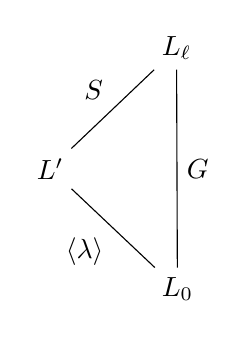
\begin{tikzpicture}
    \node (L0) {$L_0$};
    \node[above left= of L0] (Lpr) {$L'$};
    \node[above right= of Lpr] (Lm) {$L_\ell$};
    \draw (L0) edge node[right] {$G$} (Lm);
    \draw (L0) edge node[auto] {$\langle{\lambda}\rangle$} (Lpr);
    \draw (Lpr) edge node[auto] {$S$} (Lm);
\end{tikzpicture}
\end{center}
The coefficients of $\widehat{M}(T)$ being the symmetrical polynomial in the $\eta_i$, we
can see that the action of $\rho_\lambda$ will simply permute the $\widehat{\eta_i}$
leaving the coefficients unchanged. Moreover, if we take a product of less than
$r$ factor of the form $(T - \widehat{\eta_i})$, the coefficients won't be fixed
by $\rho_\lambda$, thus the polynomial is irreducible.

To finish the proof, we shall note that since $\Theta$ is in $\mathcal{O}_{L_0}$, then
by a classical result $\text{Tr}_{L_\ell/L'}(\Theta)$ is in $\mathcal{O}_{L_0}$. By
applying again the same results, we deduce that all the coefficients of $\widehat{M}(T)$
are indeed in $\mathcal{O}_{L_0}$.
\end{proof}

We are now going back to finite characteristic, $p\geq3$. Let
\begin{equation}
\mathcal{A}_0:=\F_q[X]/(\psi_{\ell,\lambda}(X))
\end{equation}
and
\begin{equation}
\mathcal{A}:=\F_p[X]/(Y^2-(X^3+AX+B),\psi_{\ell,\lambda}(X)).
\end{equation}
Let $\theta$ and $\gamma$ be the residue class of $X$ and $Y$ in $\mathcal{A}$.
We write $P = (\theta, \gamma)$ the generic point in the eigenspace of $\lambda$. 
For $o\in(\Z/\ell\Z)^{\ast}$ we define the unique polynomials 
$g_o\in\F_q$ of degree inferior to $(\ell-1)/2$ such that $g_o(\theta)= 
([o]P)_X \in\mathcal{A}$. We can then write 
\begin{equation}
\psi_{\ell,\lambda}(Z) = \prod_{i=1}^{(\ell-1)/2}{(Z - g_{\lambda^i}(\theta))}.
\end{equation}

By definition, $\ell$ is an Elkies prime of $E$, so there exists a prime 
$\mathfrak{q}$ above $\mathfrak{p}$ such that $\mathcal{O}_{L_\ell}/\mathfrak{q} =
\mathcal{A}$. We can summarize the situation with the following figure

\begin{center}
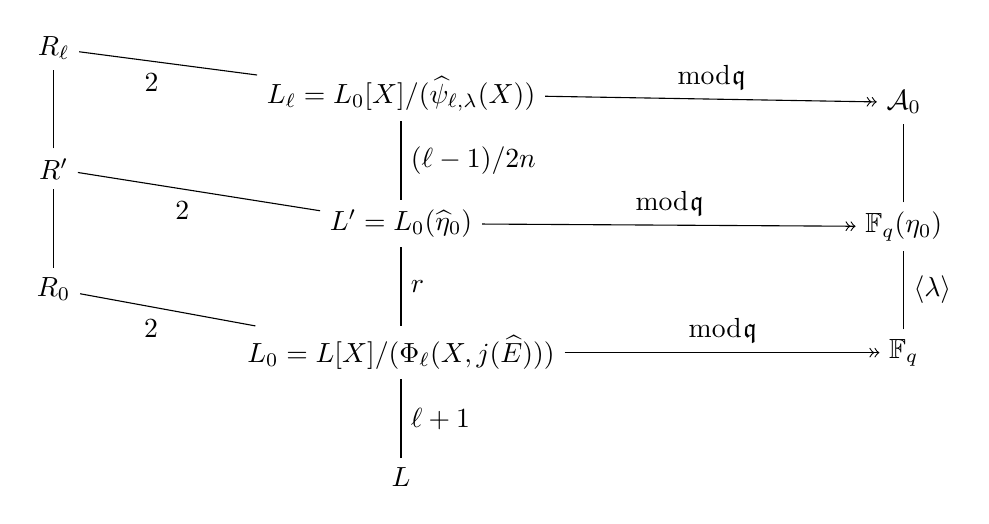
\begin{tikzpicture}
    \node (L) {$L$};
    \node[above = of L] (L0) {$L_0 = L[X]/(\Phi_{\ell}(X,j(\widehat{E})))$};
    \node[above left=0.2cm and 2cm of L0] (R0) {$R_0$};
    \node[right=4cm of L0] (Fq) {$\F_q$};
    \node[above= of L0] (Lpr) {$L' = L_0(\widehat{\eta}_0)$};
    \node[above= of Fq] (Fqa) {$\F_q(\eta_0)$};
    \node[above= of R0] (Rpr) {$R'$};
    \node[above= of Lpr] (Lm) {$L_\ell = L_0[X]/(\widehat{\psi}_{\ell,\lambda}(X))$};
    \node[above= of Rpr] (Rm) {$R_\ell$};
    \node[above= of Fqa] (A0) {$\mathcal{A}_0$};
    \draw (L) edge node[right] {$\ell+1$} (L0);
    \draw (L0) edge node[auto] {$2$} (R0);
    \draw (Lpr) edge node[auto] {$2$} (Rpr);
    \draw (Lm) edge node[auto] {$2$} (Rm);
    \draw (L0) edge node[right] {$r$} (Lpr);
    \draw (Lpr) edge node[right] {$(\ell-1)/2n$} (Lm);
    \draw (R0) edge node[auto] {} (Rpr);
    \draw (Rpr) edge node[auto] {} (Rm);
    \draw (Fq) edge node[right] {$\langle{\lambda}\rangle$} (Fqa);
    \draw (Fqa) edge node[auto] {} (A0);
    \draw[->>] (L0) edge node[auto] {$\bmod \mathfrak{q}$} (Fq);
    \draw[->>] (Lpr) edge node[auto] {$\bmod \mathfrak{q}$} (Fqa);
    \draw[->>] (Lm) edge node[auto] {$\bmod \mathfrak{q}$} (A0);
\end{tikzpicture}
\end{center}
where $\Phi_\ell(X,j(\widehat{E}))$ is an equation of the modular curve 
$X_0(\ell)$.

We can find a generator $c\in(\Z/\ell\Z)^{\ast}$ such that $\lambda = c^{r'}$
with $r'=(\ell-1)/(2n)$. Let $S:=\langle{s}\rangle$ with $s=c^r$. For 
$0\leq i<q$, we define 
\begin{equation}
\eta_i = \sum_{\sigma\in S}{g_{\sigma}(g_{\lambda^i}(\theta))}
\end{equation}
reduction modulo $\mathfrak{q}$ of $\widehat{\eta}_i$. For $\ell\geq3$ odd, the
discriminant of $\psi_\ell$ satisfies the following relation \cite{MiMoScho}
\begin{equation}
\text{Disc}(\psi_\ell)=
(-1)^{(\ell-1)/2}\ell^{(\ell^2-3)/2}(-\Delta)^{(\ell^2-1)(\ell^2-3)/24}
\end{equation}
where $\Delta$ is the discriminant of $E$. From there we can assume that the
roots of $\psi_\ell$, and consequently the roots of $\psi_{\ell,\lambda}$, are
distincts. Therefore, for $i\neq j$ we are assured that $\eta_i\neq\eta_j$ for
there would exists some linear relations between the roots of
$\psi_{\ell,\lambda}$ if that were not the case. Then, we can deduce that the 
reduction of $\widehat{M}(T)$, the minimal polynomial of $\widehat{\eta}_0$, 
is separated. As it was the case in characteristic $0$, the action of 
$\langle{\lambda}\rangle$ on the $\eta_i$ is cyclic, as a direct consequence 
the $\eta_i$ are conjugates and $M(T)$ the reduction of $\widehat{M}(T)$ is 
the minimal polynomial of $\eta_0 = \eta_\lambda(P)$ and is of degree $r$. 
This concludes the proof of the theorem.
\end{proof}

\begin{remark}
For $j=0,1728$ the results still hold. %TODO
\end{remark}

\subsection{Elliptic algorithm}

The main improvement of the elliptic variant of Rains' algorithm is the fact
that we can work directly in the extensions we are interested in. What allows
this to happen is that contrary to the roots of unity, there isn't only one
elliptic curve per extension, namely there are as many elliptic curves as there
are $j$-invariants in $\F_q$. Even more so, the use of twist of curves, which we
will be talking about later, ensures to almost always find the elliptic curve we
need for our algorithm.

 We quickly recall the situation, we have an extension $K/k$ of degree $r$,
$k'\subset K$ a subfield such that $k'\simeq k$. We wish to compute two elements 
$\alpha\in k$ and $\beta\in k'$, such that :
\begin{equation}
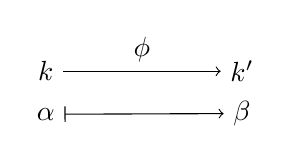
\begin{tikzpicture}
    \node (k) {$k$};
    \node[below=0.1cm of k] (alpha) {$\alpha$};
    \node[right=2cm of k] (kp) {$k'$};
    \node[below=0cm of kp] (beta) {$\beta$};

    \draw[->] (k) edge node[auto] {$\phi$} (kp);
    \draw[|->] (alpha) edge node[auto] {} (beta);

\end{tikzpicture}
\end{equation}
defines an isomorphism.
The procedure is close to the cyclotomic variant's procedure, given $k$, $K$
and $r$ we need to :
\begin{itemize}
    \item Find a prime $\ell$ and an elliptic curve $E$ satisfying the
conditions of theorem \ref{theorem:ellperiods};
    \item Take random points $P\in E(k)$ and $P'\in E(k')$ such that they are of
order $m$;
    \item Compute the elliptic periods $\alpha := \eta_{\lambda}(P)$ and $\beta
:= \eta_\lambda(P')$.
\end{itemize}
The first operation usually takes a reasonable amount of time, on exception of a
few particular case. The second operations is what will take the most ressources.
More precisely, it is the multiplication of a point on a $E(\F_{q^r})$. The last
operation also demands little time. We shall now describe in more
detail each step in detail.
    
\subsubsection{Finding an elliptic curve}
If theoritically, we always introduce the elliptic curve before finding an
Elkies prime number, in practice, we have to find a prime $\ell$ which has the good
properties and then we pick an elliptic curve for which this $\ell$ is an Elkies
prime. We shall assume $p\neq2,3$.

We need to find an integer $\ell\neq p$ such that there exist an element
$\lambda$ of order $r$ modulo $\ell$. The first condition will be that 
$r|\varphi(\ell)$. We also need that the cofactor $\varphi(\ell)/r$ is prime 
with $r$, so it ensures that $(\Z/\ell\Z)^{\ast}$ splits as we want, namely 
\begin{equation}
(\Z/\ell\Z)^{\ast}/\Aut(E)=\langle{\lambda}\rangle\times S
\end{equation}
for $S$ a subgroup of $(\Z/\ell\Z)^{\ast}$. If we chose
$\mu\in(\Z/\ell\Z)^{\ast}$ such that $\mu = q/\lambda$ of order not dividing 
$r$, then this makes $\lambda$ and $\mu$ the soon to be eigenvalues of $\pi_q$. The
fact that $\order_\ell(\mu)\not|r$ guarantees that any points on $\F_{q^r}$ will be
in the eigenspace of $\lambda$, since no subfield of $\F_{q^r}$ would contain
points of order $r$.

The next step is to find elements of $(\Z/\ell\Z)^{\ast}$ that could be used as
potential trace. Since we need $\ell$ to be an Elkies prime for the future 
elliptic curve, the charactestic polynomial of $\pi_q$ on $(\Z/\ell\Z)$ shall 
be of the form
\begin{equation}
(X - \lambda)(X - \mu) = X^2 - (\lambda + \mu)X + \lambda\mu \bmod \ell.
\end{equation}
From there, we need to find $\lambda$ and $\mu$ as we described above. Then we 
write $t:=\lambda+\mu$ and check if it is a good trace candidate using 
Hasse theorem. More precisely, we verify that $\widehat{t}$ the lift of $t$ in
$\Q$ is actually in the Hasse's bound
\begin{equation}
|\widehat{t}| \leq 2\sqrt{q}.
\end{equation}\\
In summary, we need an integer $\ell$ such that :
\begin{itemize}
    \item $\ell\neq p$ is prime,
    \item $r\mid\varphi(\ell)$ and $(\varphi(\ell)/r,r)=1$,
    \item there exists $\lambda\in(\Z/\ell\Z)^{\ast}$ such that 
\begin{equation}
\label{equation:ordeigen}
\order_\ell(\lambda) = r,\order_\ell(\dfrac{q}{\lambda}) \not| r\text{ and }|\widehat{\lambda + \dfrac{q}{\lambda}}| \leq 2\sqrt{q}.
\end{equation}
\end{itemize}

Let
\[
\mathcal{T}_\ell := \lbrace{t = \lambda + q/\lambda \bmod \ell \text{ with } \lambda\in(\Z/\ell\Z)^{\ast}
\text{ such that } \lambda \text{ satisfies 
}(\ref{equation:ordeigen})}\rbrace
\]
be the set of good trace candidates for a prime $\ell$.
To chose the right elliptic curve, we pick a $j\in\F_q$ and compute
the traces of the associated elliptic curves to check if any of them
is equal to one of the candidates in $\mathcal{T}_\ell$. See
Appendix~\ref{app:elliptic-curves} for a way of determining at once
all the traces associated to a $j$-invariant. The general procedure is as
follow.

\begin{algorithm}
    [Selecting an elliptic curve]
    \label{algorithm:selectell}
    \begin{algorithmic}[1]
    \REQUIRE $\ell$ an integer s.t. $\mathcal{T}_\ell\neq\O$, $\mathcal{T}_\ell$ 
    \ENSURE $E$ an elliptic curve with $t_E\in\mathcal{T}_\ell$
    \FOR{$j\in\F_q$}
        \STATE $E \leftarrow E(j_E = j)$ 
        \STATE $\mathcal{U} \leftarrow \mu_2, \mu_4\text{ or }\mu_6$ if 
$j_E\neq0,1728$, $j_E=1728$ or $j_E=0$ respectively.
            \FOR{$U\in\mathcal{U}$}
                \IF{$U.t_E\in\mathcal{T}_\ell$}
                    \RETURN Twist($E$, $U$)
                \ENDIF
            \ENDFOR
    \ENDFOR
    \end{algorithmic}
\end{algorithm}

To create an elliptic curve from its $j$-invariant in a finite field, we simply
use the following relations

\subsubsection{Computing the elliptic periods}

Computing the elliptic periods isn't the most complicated part of the algorithm.
Counting the points of $E/\F_{q^r}$ is directly deduced from the number of
points of $E/\F_q$ using the relation
\begin{equation}
\#E(\F_q^r)=q^r+1-(\lambda^r+\mu^r)
\end{equation}
for $\lambda, \mu$ the roots of the characteristic polynomial of $\pi_q$. To find a
point of order $\ell$ in the eigenspace of $\lambda$, we just have to find a point of
order $\ell$ in $\F_{q^r}$ thanks to the properties on the order of the eigenvalue.
The procedure is straightforward, we pick a random point in $Q\in E(\F_{q^r})$
and we compute $P = [\#E(\F_{q^r})/\ell]Q$. If $Q\neq\mathcal{O}$ then $P$ is a
point of order exactly $\ell$ in the eigenspace of $\lambda$, since $\ell$ is prime.
Depending on the $j$-invariant of $E$ the elliptic periods should be computed 
differently, see (\ref{definition:ellperiod}).
 
Practically, let $c\in(\Z/\ell\Z)^{\ast}$ be a generator such that $s = c^r$ is 
of order $\varphi(\ell)/(2n)$ in $(\Z/\ell\Z)^{\ast}/\Aut(E)$. Thus we define $S 
:= \langle{s}\rangle$, since $\lambda$ is of order $r$ in $(\Z/\ell\Z)^{\ast}$, we 
obtain the product we want
\[
(\Z/\ell\Z)^{\ast}/\Aut(E) = \langle{\lambda}\rangle\times\langle{s}\rangle
\]
Also, since all the groups are cyclic, we can rewrite the elliptic periods in a
more computable form, if we let $r_E = \#\Aut(E)$ then we have
\begin{equation}
\eta_\lambda(P) = \sum_{i = 0}^{\varphi(\ell)/r_E.r}{\left([s^i]P\right)_X^{r_E/2}}.
\end{equation}

The function can be summarized as follow

\begin{algorithm}
[Computing the elliptic periods]
\label{algorithm:compell}
    \begin{algorithmic}[1]
    \REQUIRE $K$ a finite field with $q^r$ elements, $E/\F_q$ an elliptic curve
defined over $\F_q$, $\ell$ the parameter, $r_E = \#\Aut(E)$ an integer, $c$ a 
generator of $(\Z/\ell\Z)^{\ast}$
    \ENSURE $\eta$ an elliptic period
    \STATE $\order_E\leftarrow\#E(K)$
    \STATE $\order_S \leftarrow \dfrac{\varphi(\ell)}{r_E.r}$
    \STATE $s \leftarrow c^r$
    \REPEAT
        \STATE $Q\leftarrow\text{rand}(E(K))$
        \STATE $P\leftarrow[\dfrac{\order_E}{\ell}]Q$
    \UNTIL{$P\neq\mathcal{O}$}
    \STATE $\eta\leftarrow\sum_{i=0}^{\order_S}{\left([s^i]P\right)_X^{r_E/2}}$
    \RETURN $\eta$
    \end{algorithmic}
\end{algorithm}

\begin{remark}
A simple fact in favor of taking the automorphism group of $E$ into account is
easily illustrated in the case $j\neq0,1728$. In this case, $\Aut(E) =
\lbrace{\pm1}\rbrace$ and since $P_X = (-P)_X$, we would be actually summing the
same element two times; which isn't necessary to what we do.

However, another more pathological issue arises when we are working on the
specific case $j = 0$ or $1728$. For example, if we consider the case $j =
1728$, we know that an element of $\sigma\in\Aut(E)$ acts as follow
\[
\sigma : (x,y) \mapsto (-x, iy)
\]
Therefore, we can end up summing points with opposites abscissas, resulting in a
$0$ sum, which isn't of great interest. A counter to this phenomenon is to
square the abscissas. The same happens with the case $j = 0$, only this time
$3$rd roots of unity are invovled instead of $\pm1$.
\end{remark}

\subsubsection{Isomorphism algorithm}

We recall that $k_1\simeq\F_q[X]/(f)$ and $k_2\simeq\F_q[Y]/(g)$. Then using the
previous algorithms, we compute a period elliptic in each field extension. By
the theorem \ref{}, they define an isomorphism. Therefore we can state the
complete elliptic variants of Rains' algorithm.

\begin{algorithm}
[Elliptic variants of Rains' algorithm]
\label{algorithm:rainsell}
    \begin{algorithmic}[1]
    \REQUIRE $k_1$, $k_2$, $\F_q$
    \ENSURE $\eta_1\in k_1$, $\eta_2\in k_2$ two elements defining an
isomorphism
    \STATE Find $\ell$ s.t. $\mathcal{T}_\ell\neq\emptyset$
    \STATE Compute $g$ a generator of $\F_{q^n}^{\times}$
    \STATE Find $E$ using algorithm (\ref{algorithm:selectell})
    \STATE Compute $c$ a generator of $(\Z/m\Z)^{\times}$
    \STATE Compute $\eta_1$ in $k_1$ using algorithm (\ref{algorithm:compell})
    \STATE Compute $\eta_2$ in $k_2$ using algorithm (\ref{algorithm:compell})
    \RETURN $\eta_1, \eta_2$
    \end{algorithmic}
\end{algorithm}

\subsection{Complexity analysis}

\section{Algorithm selection}
\label{sec:selection}

\section{Experimental Results}

%%%%%%%%%%%%%%%%%%%%%%%%%%%%%%%%%%
%%%%%%%%%%%%%%%%%%%%%%%%%%%%%%%%%%

\part{Embedding evaluation}
\label{part:eval}


\subsubsection{Linear algebra}

Once $\beta \in K$ has been computed as a polynomial in $Y$,
one can compute the powers
$\beta^i = \sum_{j=0}^{n-1} m_{i,j} Y^j$
for $i \in \{0, \ldots, n-1\}$ and build a matrix
$M = \{m_{i, j}\}_{0\leq i \leq m-1, 0 \leq j \leq n -1}$
representing $\phi$.
This is trivially done in $O(m)$ operations in $K$.
For $\gamma = \sum_{i = 0}^{m - 1} c_i X^i \in k$,
$\phi(\gamma)$ can then be computed by a
matrix-vector multiplication in $O(m n)$ operations in $\F_q$.

Together, the second and third questions are the inverse image problem.
They can be answered by first computing 
an LU or similar matrix decompostions of $M$
in $O((n (m)^{\omega - 1})$ operations in $\F_q$.
Answering the second and third questions together is then
an easy matter.

Note that if $m = n$, that is if $k$ and $K$ are
isomorphic, then the second question is trivial.
For the third one, the inverse
the inverse $M^{-1}$ of $M$ representing $\phi^{-1}$
can be deduced from an an LU or similar matrix decompostions of $M$.
For $\delta \in K$, $\phi^{-1}(\delta)$ can then be computed by a
matrix-vector multiplication in $O(m^2)$ in $\F_q$.

\subsubsection{Modular composition}

As an alternative to using linear algebra,
$\phi(\gamma)$ can be computed directly using modular composition
as $\beta(\gamma) \pmod{g}$ in $\MC(n)$ operations in $\F_q$.

The second question can be answered by performing a modular
exponentiation to check that $\gamma^{q^{m}} = 1$
naively in $O(m \log q)$ operations in $K$
or in $O(\log q)$ operations in $K$ plus
$O(\log m) \MC(n)$ operations in $\F_q$ using modular composition.

The second and third questions can be answered using
dual bases and power projection/transposed modular composition
to express $\delta \in K$ as a polynomial in $\beta$ in
$\MC(n)$ operations in $\F_q$.


%%%%%%%%%%%%%%%%%%%%%%%%%%%%%%%%%%

\section{Algorithms specific to normal bases}

%%%%%%%%%%%%%%%%%%%%%%%%%%%%%%%%%%

\section{Monomial-dual bases pairs}

%%%%%%%%%%%%%%%%%%%%%%%%%%%%%%%%%%

\section{Experimental results}

%%%%%%%%%%%%%%%%%%%%%%%%%%%%%%%%%%

\section{Conclusion}

%%%%%%%%%%%%%%%%%%%%%%%%%%%%%%%%%%
%%%%%%%%%%%%%%%%%%%%%%%%%%%%%%%%%%

\appendix
\part*{Appendices}
\addcontentsline{toc}{part}{Appendices}

%%%%%%%%%%%%%%%%%%%%%%%%%%%%%%%%%%

\section{Elliptic curves}
\label{app:elliptic-curves}

Recall that two elliptic curves $E$ and $E'$ over a field $k$ are said
to be \emph{isomorphic} if there exists a linear change of variables
with coefficients in $k$ sending one onto the other. If $E$ and $E'$
are isomorphic over $\bar{k}$, but not over $k$, they are said to be
\emph{twists} of each other. A twist is said to be quadratic
(resp. cubic, quartic, sextic), if $E$ and $E'$ become isomorphic over
a quadratic (resp. cubic, quartic, sextic) extension of $k$. Most
elliptic curves only have quadratic twists; elliptic curves with
$j=0,1728$ may have cubic, quartic and sextic twists. See~\cite{Sil}.

We now give a proposition relating the number of points of an elliptic
curve over a finite field with the number of points of its twists.  In
the case of quadratic twists, this proposition simply states that $E$
and $E'$ have opposite trace, a well known fact.

\begin{proposition}
  \label{proposition:twisttrace}
  Let $E$ be an ordinary elliptic curve defined over a finite field
  $\F_q$ of characteristic $p$, and denote by $t$ the trace of its
  frobenius endomorphism.

  Let $u\in\bar{\F}_q$ such that $u^{q-1}$ is in the prime field
  $\F_p\subset\F_q$. Define a curve $E^u$ and an isomorphism
  $\upsilon$ of elliptic curves by
  \begin{equation*}
    \begin{aligned}
      \upsilon : E &\to E^u,\\
      (x,y) &\mapsto (u^2x,u^3y).
    \end{aligned}
  \end{equation*}
  
  If $E^u$ is defined over $\F_q$, the trace $t_u$ of its frobenius
  endomorphism is such that $t/t_u=U\bmod q$, where
  \begin{enumerate}[a)]
  \item $U$ is an element of $\Z/q\Z$ of the same multiplicative order
    as $u^{1-q}\in\F_q$, and
  \item $U=u^{1-q}\mod p$.
  \end{enumerate}
\end{proposition}
\begin{proof}
  Observe that if $E^u$ is a quadratic (resp. cubic, quartic, sextic)
  twist of $E$, then $u^{q-1}$ has multiplicative order $2$
  (resp. $3,4,6$). Furthermore, since $E$ is ordinary, $u^{q-1}$ is in
  the prime field $\F_p$ and it defines a curve automorphism
  \begin{equation*}
    \upsilon^{q-1}:(x,y)\mapsto(u^{2q-2}x,u^{3q-3}y).
  \end{equation*}
  Any twist arises this way (see~\cite{Sil}).

  Denote by $\pi$ and $\pi_u$ the frobenius endomorphisms of $E$
  and $E^u$ respectively. They satisfy the equations
  \begin{equation}
    \label{eq:frob-char-twist}
    \pi^2 - [t]\pi + [q] = 0, \qquad \pi_u^2 - [t_u]\pi_u + [q] = 0,
  \end{equation}
  where $[m]$ denotes multiplication by $m$ on the elliptic curves. By
  straightforward calculation, we also verify that they satisfy the
  commutative diagram
  \begin{equation*}
    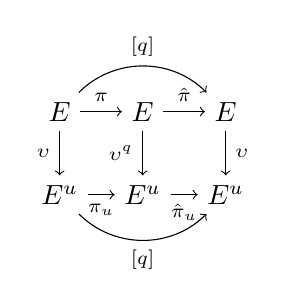
\begin{tikzpicture}[node distance=3em]
      \node(E){$E$};
      \node[right of=E](E2){$E$};
      \node[right of=E2](E3){$E$};
      \node[below of=E](Eu){$E^u$};
      \node[right of=Eu](Eu2){$E^u$};
      \node[right of=Eu2](Eu3){$E^u$};

      \draw[->,auto,font=\scriptsize]
      (E) edge node[swap]{$\upsilon$} (Eu)
          edge node{$\pi$} (E2)
          edge[bend left=45] node{$[q]$} (E3)
      (Eu) edge node[swap]{$\pi_u$} (Eu2)
           edge[bend right=45] node[swap]{$[q]$} (Eu3)
      (E2) edge node[swap]{$\upsilon^q$} (Eu2)
           edge node{$\hat\pi$} (E3)
      (Eu2) edge node[swap]{$\hat\pi_u$} (Eu3)
      (E3) edge node{$\upsilon$} (Eu3);
    \end{tikzpicture}
  \end{equation*}
  where we denote by $\upsilon^q$ the isomorphism
  $(x,y)\mapsto(u^{2q}x,u^{3q}y)$, and by $\hat\pi,\hat\pi_u$ the dual isogenies
  to $\pi,\pi_u$.

  Now we restrict the maps above to the $q$-torsion subgroups of $E$
  and $E^u$. Since the curves are ordinary, these subgroups are cyclic
  of order $q$, and the maps act as scalar multiplication on the
  points. In particular, we deduce from Eq.~\eqref{eq:frob-char-twist} that 
  \begin{equation*}
    \pi = [t \bmod q], \qquad \pi_u = [t_u \bmod q].
  \end{equation*}
  Hence, from the diagram we obtain
  \begin{equation*}
    [t] = \upsilon^{-q}\circ[t_u]\circ\upsilon \mod q.
  \end{equation*}

  Notice that $\upsilon^{-q}$ can be decomposed as
  $\upsilon^{-1}\circ\upsilon^{1-q}$, where $\upsilon^{1-q}$ is an
  automorphism of $E^u$ by hypothesis. $\upsilon^{1-q}$ also acts on
  the $q$-torsion points as a scalar in $\Z/q\Z$, that we shall denote
  by $U$. It is evident that the multiplicative order of $U$ in $\Z/q\Z$
  is the same as that of $u^{1-q}$ in $\F_p$. Then
  \begin{equation*}
    [t] = \upsilon^{-1}\circ[Ut_u]\circ\upsilon.
  \end{equation*}
  But $\upsilon$ is an isomorphism, thus it commutes with scalar
  multiplication, and we conclude that $t=Ut_u\bmod q$.

  If $u^{1-q}=\pm1$, we are done. When the order of $u^{1-q}$ is $3,4$
  or $6$, we still have to determine which of the cubic, fourth, sixth
  roots of unity in $\Z/q\Z$ corresponds to $U$.

  Using the diagram above, we decompose
  Eq.~\eqref{eq:frob-char-twist} as
  \begin{equation*}
    \hat\pi\circ\pi = [t]\pi - \pi^2,
  \end{equation*}
  and similarly for $E^u$. Hence, from the diagram again,
  \begin{equation*}
    [t] - \pi = \hat\pi = \upsilon^{-1}\circ\hat\pi_u\circ\upsilon^q 
    =  \upsilon^{-1}\circ([t_u] - \pi_u)\circ\upsilon^q.
  \end{equation*}
  Let now $\omega$ be the invariant differential of $E$. We have
  \begin{equation*}
    ([t]-\pi^2)^\ast\omega = t\omega\in\Omega_E
  \end{equation*}
  because $\pi$ is inserparable. On the other hand, if we let
  $\omega_u$ be the invariant differential of $E^u$, we have
  \begin{multline*}
    (\upsilon^{-1}\circ([t_u] - \pi_u)\circ\upsilon^q)^\ast\omega =
    (\upsilon^{-1}\circ([t_u] - \pi_u)\circ\upsilon^{q-1})^\ast\omega_u =\\
    (\upsilon^{-1}\circ([t_u] - \pi_u))^\ast u^{1-q}\omega_u =
    (\upsilon^{-1})^\ast t_uu^{1-q}\omega_u =
    t_uu^{1-q}\omega.
  \end{multline*}
  Hence $t = t_uu^{1-q} \bmod p$.
\end{proof}

\todo{Give a similar proposition for supersingular curves (see, e.g.,
  Menezes-Okamoto-Vanstone)}

%%%%%%%%%%%%%%%%%%%%%%%%%%%%%%%%%%
%%%%%%%%%%%%%%%%%%%%%%%%%%%%%%%%%%

\bibliographystyle{plain}
\bibliography{defeo}

\end{document}


% Local Variables:
% ispell-local-dictionary:"american"
% End:

%  LocalWords:  isomorphism cyclotomic coprime subfield
